\documentclass[twoside]{book}

% Packages required by doxygen
\usepackage{calc}
\usepackage{doxygen}
\usepackage{graphicx}
\usepackage[utf8]{inputenc}
\usepackage{makeidx}
\usepackage{multicol}
\usepackage{multirow}
\usepackage{textcomp}
\usepackage[table]{xcolor}

% Font selection
\usepackage[T1]{fontenc}
\usepackage{mathptmx}
\usepackage[scaled=.90]{helvet}
\usepackage{courier}
\usepackage{amssymb}
\usepackage{sectsty}
\renewcommand{\familydefault}{\sfdefault}
\allsectionsfont{%
  \fontseries{bc}\selectfont%
  \color{darkgray}%
}
\renewcommand{\DoxyLabelFont}{%
  \fontseries{bc}\selectfont%
  \color{darkgray}%
}

% Page & text layout
\usepackage{geometry}
\geometry{%
  a4paper,%
  top=2.5cm,%
  bottom=2.5cm,%
  left=2.5cm,%
  right=2.5cm%
}
\tolerance=750
\hfuzz=15pt
\hbadness=750
\setlength{\emergencystretch}{15pt}
\setlength{\parindent}{0cm}
\setlength{\parskip}{0.2cm}
\makeatletter
\renewcommand{\paragraph}{%
  \@startsection{paragraph}{4}{0ex}{-1.0ex}{1.0ex}{%
    \normalfont\normalsize\bfseries\SS@parafont%
  }%
}
\renewcommand{\subparagraph}{%
  \@startsection{subparagraph}{5}{0ex}{-1.0ex}{1.0ex}{%
    \normalfont\normalsize\bfseries\SS@subparafont%
  }%
}
\makeatother

% Headers & footers
\usepackage{fancyhdr}
\pagestyle{fancyplain}
\fancyhead[LE]{\fancyplain{}{\bfseries\thepage}}
\fancyhead[CE]{\fancyplain{}{}}
\fancyhead[RE]{\fancyplain{}{\bfseries\leftmark}}
\fancyhead[LO]{\fancyplain{}{\bfseries\rightmark}}
\fancyhead[CO]{\fancyplain{}{}}
\fancyhead[RO]{\fancyplain{}{\bfseries\thepage}}
\fancyfoot[LE]{\fancyplain{}{}}
\fancyfoot[CE]{\fancyplain{}{}}
\fancyfoot[RE]{\fancyplain{}{\bfseries\scriptsize Generated on Wed Dec 3 2014 18\-:03\-:05 for Deeto by Doxygen }}
\fancyfoot[LO]{\fancyplain{}{\bfseries\scriptsize Generated on Wed Dec 3 2014 18\-:03\-:05 for Deeto by Doxygen }}
\fancyfoot[CO]{\fancyplain{}{}}
\fancyfoot[RO]{\fancyplain{}{}}
\renewcommand{\footrulewidth}{0.4pt}
\renewcommand{\chaptermark}[1]{%
  \markboth{#1}{}%
}
\renewcommand{\sectionmark}[1]{%
  \markright{\thesection\ #1}%
}

% Indices & bibliography
\usepackage{natbib}
\usepackage[titles]{tocloft}
\setcounter{tocdepth}{3}
\setcounter{secnumdepth}{5}
\makeindex

% Hyperlinks (required, but should be loaded last)
\usepackage{ifpdf}
\ifpdf
  \usepackage[pdftex,pagebackref=true]{hyperref}
\else
  \usepackage[ps2pdf,pagebackref=true]{hyperref}
\fi
\hypersetup{%
  colorlinks=true,%
  linkcolor=blue,%
  citecolor=blue,%
  unicode%
}

% Custom commands
\newcommand{\clearemptydoublepage}{%
  \newpage{\pagestyle{empty}\cleardoublepage}%
}


%===== C O N T E N T S =====

\begin{document}

% Titlepage & ToC
\hypersetup{pageanchor=false}
\pagenumbering{roman}
\begin{titlepage}
\vspace*{7cm}
\begin{center}%
{\Large Deeto }\\
\vspace*{1cm}
{\large Generated by Doxygen 1.8.6}\\
\vspace*{0.5cm}
{\small Wed Dec 3 2014 18:03:05}\\
\end{center}
\end{titlepage}
\clearemptydoublepage
\tableofcontents
\clearemptydoublepage
\pagenumbering{arabic}
\hypersetup{pageanchor=true}

%--- Begin generated contents ---
\chapter{Hierarchical Index}
\section{Class Hierarchy}
This inheritance list is sorted roughly, but not completely, alphabetically\-:\begin{DoxyCompactList}
\item \contentsline{section}{Abstract\-Writer}{\pageref{classAbstractWriter}}{}
\begin{DoxyCompactList}
\item \contentsline{section}{F\-C\-S\-V\-Writer}{\pageref{classFCSVWriter}}{}
\item \contentsline{section}{V\-T\-K\-Writer}{\pageref{classVTKWriter}}{}
\end{DoxyCompactList}
\item \contentsline{section}{Anatomical\-Patch\-Builder$<$ class T $>$}{\pageref{classAnatomicalPatchBuilder_3_01class_01T_01_4}}{}
\item \contentsline{section}{Clinical\-Frame}{\pageref{classClinicalFrame}}{}
\item \contentsline{section}{Contact\-Constructor}{\pageref{classContactConstructor}}{}
\item \contentsline{section}{Electrode}{\pageref{classElectrode}}{}
\item \contentsline{section}{Electrode\-Model}{\pageref{classElectrodeModel}}{}
\item \contentsline{section}{F\-C\-S\-V\-Reader}{\pageref{classFCSVReader}}{}
\item \contentsline{section}{G\-M\-P\-I\-Estimator}{\pageref{classGMPIEstimator}}{}
\item \contentsline{section}{V\-T\-K\-Model\-Constructor}{\pageref{classVTKModelConstructor}}{}
\end{DoxyCompactList}

\chapter{Class Index}
\section{Class List}
Here are the classes, structs, unions and interfaces with brief descriptions\-:\begin{DoxyCompactList}
\item\contentsline{section}{\hyperlink{classAbstractWriter}{Abstract\-Writer} }{\pageref{classAbstractWriter}}{}
\item\contentsline{section}{\hyperlink{classAnatomicalPatchBuilder_3_01class_01T_01_4}{Anatomical\-Patch\-Builder$<$ class T $>$} }{\pageref{classAnatomicalPatchBuilder_3_01class_01T_01_4}}{}
\item\contentsline{section}{\hyperlink{classClinicalFrame}{Clinical\-Frame} }{\pageref{classClinicalFrame}}{}
\item\contentsline{section}{\hyperlink{classContactConstructor}{Contact\-Constructor} }{\pageref{classContactConstructor}}{}
\item\contentsline{section}{\hyperlink{classElectrode}{Electrode} }{\pageref{classElectrode}}{}
\item\contentsline{section}{\hyperlink{classElectrodeModel}{Electrode\-Model} }{\pageref{classElectrodeModel}}{}
\item\contentsline{section}{\hyperlink{classFCSVReader}{F\-C\-S\-V\-Reader} }{\pageref{classFCSVReader}}{}
\item\contentsline{section}{\hyperlink{classFCSVWriter}{F\-C\-S\-V\-Writer} }{\pageref{classFCSVWriter}}{}
\item\contentsline{section}{\hyperlink{classGMPIEstimator}{G\-M\-P\-I\-Estimator} }{\pageref{classGMPIEstimator}}{}
\item\contentsline{section}{\hyperlink{classVTKModelConstructor}{V\-T\-K\-Model\-Constructor} }{\pageref{classVTKModelConstructor}}{}
\item\contentsline{section}{\hyperlink{classVTKWriter}{V\-T\-K\-Writer} }{\pageref{classVTKWriter}}{}
\end{DoxyCompactList}

\chapter{File Index}
\section{File List}
Here is a list of all files with brief descriptions\-:\begin{DoxyCompactList}
\item\contentsline{section}{\hyperlink{AbstractWriter_8h}{Abstract\-Writer.\-h} }{\pageref{AbstractWriter_8h}}{}
\item\contentsline{section}{\hyperlink{AnatomicalPatchBuilder_8h}{Anatomical\-Patch\-Builder.\-h} }{\pageref{AnatomicalPatchBuilder_8h}}{}
\item\contentsline{section}{\hyperlink{ClinicalFrame_8h}{Clinical\-Frame.\-h} }{\pageref{ClinicalFrame_8h}}{}
\item\contentsline{section}{\hyperlink{ContactConstructor_8h}{Contact\-Constructor.\-h} }{\pageref{ContactConstructor_8h}}{}
\item\contentsline{section}{\hyperlink{Definitions_8h}{Definitions.\-h} }{\pageref{Definitions_8h}}{}
\item\contentsline{section}{\hyperlink{Electrode_8h}{Electrode.\-h} }{\pageref{Electrode_8h}}{}
\item\contentsline{section}{\hyperlink{ElectrodeModel_8h}{Electrode\-Model.\-h} }{\pageref{ElectrodeModel_8h}}{}
\item\contentsline{section}{\hyperlink{FCSVReader_8h}{F\-C\-S\-V\-Reader.\-h} }{\pageref{FCSVReader_8h}}{}
\item\contentsline{section}{\hyperlink{FCSVWriter_8h}{F\-C\-S\-V\-Writer.\-h} }{\pageref{FCSVWriter_8h}}{}
\item\contentsline{section}{\hyperlink{GMPIEstimator_8h}{G\-M\-P\-I\-Estimator.\-h} }{\pageref{GMPIEstimator_8h}}{}
\item\contentsline{section}{\hyperlink{VTKModelConstructor_8h}{V\-T\-K\-Model\-Constructor.\-h} }{\pageref{VTKModelConstructor_8h}}{}
\item\contentsline{section}{\hyperlink{VTKWriter_8h}{V\-T\-K\-Writer.\-h} }{\pageref{VTKWriter_8h}}{}
\end{DoxyCompactList}

\chapter{Class Documentation}
\hypertarget{classAbstractWriter}{\section{Abstract\-Writer Class Reference}
\label{classAbstractWriter}\index{Abstract\-Writer@{Abstract\-Writer}}
}


{\ttfamily \#include $<$Abstract\-Writer.\-h$>$}



Inheritance diagram for Abstract\-Writer\-:
\nopagebreak
\begin{figure}[H]
\begin{center}
\leavevmode
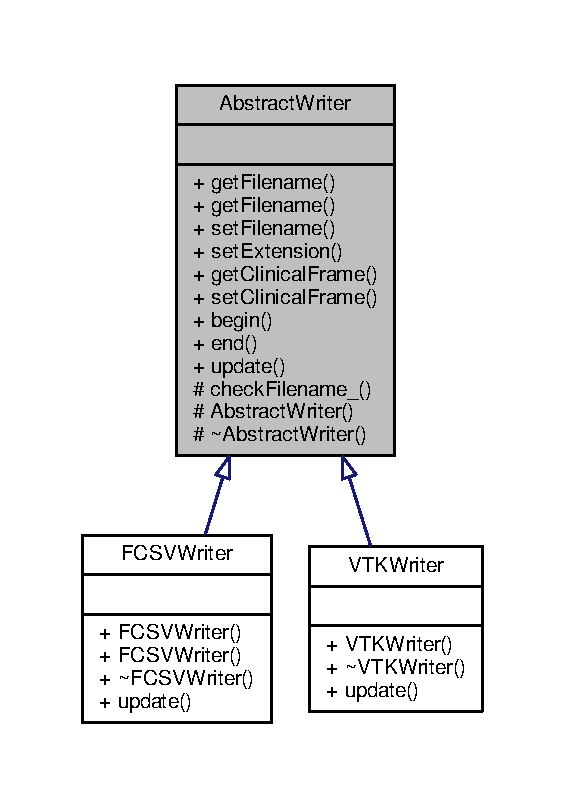
\includegraphics[width=271pt]{classAbstractWriter__inherit__graph}
\end{center}
\end{figure}


Collaboration diagram for Abstract\-Writer\-:
\nopagebreak
\begin{figure}[H]
\begin{center}
\leavevmode
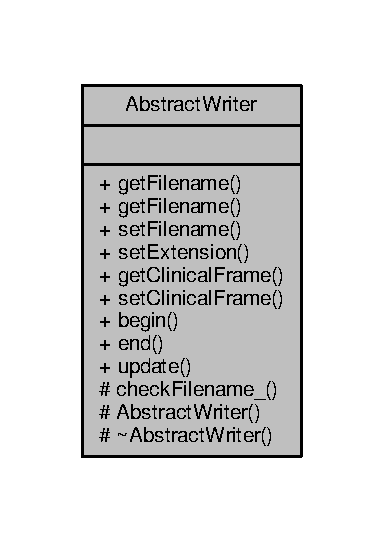
\includegraphics[width=184pt]{classAbstractWriter__coll__graph}
\end{center}
\end{figure}
\subsection*{Public Member Functions}
\begin{DoxyCompactItemize}
\item 
const string \hyperlink{classAbstractWriter_ae2cdd50fc9b39e6ded80bb7d9cea55b0}{get\-Filename} () const 
\item 
void \hyperlink{classAbstractWriter_ab743677bd3db72113a57188093425306}{get\-Filename} (string filename) const 
\item 
void \hyperlink{classAbstractWriter_ac13745f7801378b8231bb54c45490dbe}{set\-Filename} (string filename)
\item 
void \hyperlink{classAbstractWriter_ab1bb7069f6b7886cb46718fb4c9eff5c}{set\-Extension} (string ext)
\item 
const \hyperlink{classClinicalFrame}{Clinical\-Frame} $\ast$ \hyperlink{classAbstractWriter_ae43ecbb0fbb883629ea44a7a7c906e1a}{get\-Clinical\-Frame} (void) const 
\item 
void \hyperlink{classAbstractWriter_a64827ba205471ae1d9fa9e5d890f3335}{set\-Clinical\-Frame} (\hyperlink{classClinicalFrame}{Clinical\-Frame} $\ast$cf)
\item 
\hyperlink{classClinicalFrame_ab741d0da22f344965de240de63c8a381}{Clinical\-Frame\-::\-Const\-Electrode\-Iterator} \hyperlink{classAbstractWriter_a02d123991818324034406e38c30bce1d}{begin} (void) const 
\item 
\hyperlink{classClinicalFrame_ab741d0da22f344965de240de63c8a381}{Clinical\-Frame\-::\-Const\-Electrode\-Iterator} \hyperlink{classAbstractWriter_a21776d6dc864b6cdadd49791ccfc6677}{end} (void) const 
\item 
virtual int \hyperlink{classAbstractWriter_ae3d1e946840352b28b092902664a1115}{update} ()=0
\end{DoxyCompactItemize}
\subsection*{Protected Member Functions}
\begin{DoxyCompactItemize}
\item 
void \hyperlink{classAbstractWriter_a75c621b83faaa753dddcb24d45f96d44}{check\-Filename\-\_\-} (void)
\item 
\hyperlink{classAbstractWriter_a56e1e861dc5b9ec7d6de79e6701fd06d}{Abstract\-Writer} ()
\item 
virtual \hyperlink{classAbstractWriter_a8d2dcb8b137bc04f8c22ec57ac59ed4e}{$\sim$\-Abstract\-Writer} ()
\end{DoxyCompactItemize}


\subsection{Detailed Description}
\hyperlink{classAbstractWriter}{Abstract\-Writer} class This class is the base class for each writer. It takes care of filename consistency and it holds the \hyperlink{classClinicalFrame}{Clinical\-Frame} pointer. 

\subsection{Constructor \& Destructor Documentation}
\hypertarget{classAbstractWriter_a56e1e861dc5b9ec7d6de79e6701fd06d}{\index{Abstract\-Writer@{Abstract\-Writer}!Abstract\-Writer@{Abstract\-Writer}}
\index{Abstract\-Writer@{Abstract\-Writer}!AbstractWriter@{Abstract\-Writer}}
\subsubsection[{Abstract\-Writer}]{\setlength{\rightskip}{0pt plus 5cm}Abstract\-Writer\-::\-Abstract\-Writer (
\begin{DoxyParamCaption}
{}
\end{DoxyParamCaption}
)\hspace{0.3cm}{\ttfamily [inline]}, {\ttfamily [protected]}}}\label{classAbstractWriter_a56e1e861dc5b9ec7d6de79e6701fd06d}
Purposely proteced since it is supposed to be istantiated only by its child \hypertarget{classAbstractWriter_a8d2dcb8b137bc04f8c22ec57ac59ed4e}{\index{Abstract\-Writer@{Abstract\-Writer}!$\sim$\-Abstract\-Writer@{$\sim$\-Abstract\-Writer}}
\index{$\sim$\-Abstract\-Writer@{$\sim$\-Abstract\-Writer}!AbstractWriter@{Abstract\-Writer}}
\subsubsection[{$\sim$\-Abstract\-Writer}]{\setlength{\rightskip}{0pt plus 5cm}virtual Abstract\-Writer\-::$\sim$\-Abstract\-Writer (
\begin{DoxyParamCaption}
{}
\end{DoxyParamCaption}
)\hspace{0.3cm}{\ttfamily [inline]}, {\ttfamily [protected]}, {\ttfamily [virtual]}}}\label{classAbstractWriter_a8d2dcb8b137bc04f8c22ec57ac59ed4e}
It sets the Clinical\-Frame$\ast$ to N\-U\-L\-L upon call 

\subsection{Member Function Documentation}
\hypertarget{classAbstractWriter_a02d123991818324034406e38c30bce1d}{\index{Abstract\-Writer@{Abstract\-Writer}!begin@{begin}}
\index{begin@{begin}!AbstractWriter@{Abstract\-Writer}}
\subsubsection[{begin}]{\setlength{\rightskip}{0pt plus 5cm}{\bf Clinical\-Frame\-::\-Const\-Electrode\-Iterator} Abstract\-Writer\-::begin (
\begin{DoxyParamCaption}
\item[{void}]{}
\end{DoxyParamCaption}
) const\hspace{0.3cm}{\ttfamily [inline]}}}\label{classAbstractWriter_a02d123991818324034406e38c30bce1d}
returns the head of Const\-Electrode\-Iterator to navigate the \hyperlink{classClinicalFrame}{Clinical\-Frame} implant details \hypertarget{classAbstractWriter_a75c621b83faaa753dddcb24d45f96d44}{\index{Abstract\-Writer@{Abstract\-Writer}!check\-Filename\-\_\-@{check\-Filename\-\_\-}}
\index{check\-Filename\-\_\-@{check\-Filename\-\_\-}!AbstractWriter@{Abstract\-Writer}}
\subsubsection[{check\-Filename\-\_\-}]{\setlength{\rightskip}{0pt plus 5cm}void Abstract\-Writer\-::check\-Filename\-\_\- (
\begin{DoxyParamCaption}
\item[{void}]{}
\end{DoxyParamCaption}
)\hspace{0.3cm}{\ttfamily [inline]}, {\ttfamily [protected]}}}\label{classAbstractWriter_a75c621b83faaa753dddcb24d45f96d44}
appends correct extension to filename depending on which subclass has been istantiated \hypertarget{classAbstractWriter_a21776d6dc864b6cdadd49791ccfc6677}{\index{Abstract\-Writer@{Abstract\-Writer}!end@{end}}
\index{end@{end}!AbstractWriter@{Abstract\-Writer}}
\subsubsection[{end}]{\setlength{\rightskip}{0pt plus 5cm}{\bf Clinical\-Frame\-::\-Const\-Electrode\-Iterator} Abstract\-Writer\-::end (
\begin{DoxyParamCaption}
\item[{void}]{}
\end{DoxyParamCaption}
) const\hspace{0.3cm}{\ttfamily [inline]}}}\label{classAbstractWriter_a21776d6dc864b6cdadd49791ccfc6677}
returns the tail fo Const\-Electrode\-Iterator \hypertarget{classAbstractWriter_ae43ecbb0fbb883629ea44a7a7c906e1a}{\index{Abstract\-Writer@{Abstract\-Writer}!get\-Clinical\-Frame@{get\-Clinical\-Frame}}
\index{get\-Clinical\-Frame@{get\-Clinical\-Frame}!AbstractWriter@{Abstract\-Writer}}
\subsubsection[{get\-Clinical\-Frame}]{\setlength{\rightskip}{0pt plus 5cm}const {\bf Clinical\-Frame}$\ast$ Abstract\-Writer\-::get\-Clinical\-Frame (
\begin{DoxyParamCaption}
\item[{void}]{}
\end{DoxyParamCaption}
) const\hspace{0.3cm}{\ttfamily [inline]}}}\label{classAbstractWriter_ae43ecbb0fbb883629ea44a7a7c906e1a}
\hypertarget{classAbstractWriter_ae2cdd50fc9b39e6ded80bb7d9cea55b0}{\index{Abstract\-Writer@{Abstract\-Writer}!get\-Filename@{get\-Filename}}
\index{get\-Filename@{get\-Filename}!AbstractWriter@{Abstract\-Writer}}
\subsubsection[{get\-Filename}]{\setlength{\rightskip}{0pt plus 5cm}const string Abstract\-Writer\-::get\-Filename (
\begin{DoxyParamCaption}
{}
\end{DoxyParamCaption}
) const\hspace{0.3cm}{\ttfamily [inline]}}}\label{classAbstractWriter_ae2cdd50fc9b39e6ded80bb7d9cea55b0}
\hypertarget{classAbstractWriter_ab743677bd3db72113a57188093425306}{\index{Abstract\-Writer@{Abstract\-Writer}!get\-Filename@{get\-Filename}}
\index{get\-Filename@{get\-Filename}!AbstractWriter@{Abstract\-Writer}}
\subsubsection[{get\-Filename}]{\setlength{\rightskip}{0pt plus 5cm}void Abstract\-Writer\-::get\-Filename (
\begin{DoxyParamCaption}
\item[{string}]{filename}
\end{DoxyParamCaption}
) const\hspace{0.3cm}{\ttfamily [inline]}}}\label{classAbstractWriter_ab743677bd3db72113a57188093425306}
\hypertarget{classAbstractWriter_a64827ba205471ae1d9fa9e5d890f3335}{\index{Abstract\-Writer@{Abstract\-Writer}!set\-Clinical\-Frame@{set\-Clinical\-Frame}}
\index{set\-Clinical\-Frame@{set\-Clinical\-Frame}!AbstractWriter@{Abstract\-Writer}}
\subsubsection[{set\-Clinical\-Frame}]{\setlength{\rightskip}{0pt plus 5cm}void Abstract\-Writer\-::set\-Clinical\-Frame (
\begin{DoxyParamCaption}
\item[{{\bf Clinical\-Frame} $\ast$}]{cf}
\end{DoxyParamCaption}
)\hspace{0.3cm}{\ttfamily [inline]}}}\label{classAbstractWriter_a64827ba205471ae1d9fa9e5d890f3335}
\hypertarget{classAbstractWriter_ab1bb7069f6b7886cb46718fb4c9eff5c}{\index{Abstract\-Writer@{Abstract\-Writer}!set\-Extension@{set\-Extension}}
\index{set\-Extension@{set\-Extension}!AbstractWriter@{Abstract\-Writer}}
\subsubsection[{set\-Extension}]{\setlength{\rightskip}{0pt plus 5cm}void Abstract\-Writer\-::set\-Extension (
\begin{DoxyParamCaption}
\item[{string}]{ext}
\end{DoxyParamCaption}
)\hspace{0.3cm}{\ttfamily [inline]}}}\label{classAbstractWriter_ab1bb7069f6b7886cb46718fb4c9eff5c}
\hypertarget{classAbstractWriter_ac13745f7801378b8231bb54c45490dbe}{\index{Abstract\-Writer@{Abstract\-Writer}!set\-Filename@{set\-Filename}}
\index{set\-Filename@{set\-Filename}!AbstractWriter@{Abstract\-Writer}}
\subsubsection[{set\-Filename}]{\setlength{\rightskip}{0pt plus 5cm}void Abstract\-Writer\-::set\-Filename (
\begin{DoxyParamCaption}
\item[{string}]{filename}
\end{DoxyParamCaption}
)\hspace{0.3cm}{\ttfamily [inline]}}}\label{classAbstractWriter_ac13745f7801378b8231bb54c45490dbe}
\hypertarget{classAbstractWriter_ae3d1e946840352b28b092902664a1115}{\index{Abstract\-Writer@{Abstract\-Writer}!update@{update}}
\index{update@{update}!AbstractWriter@{Abstract\-Writer}}
\subsubsection[{update}]{\setlength{\rightskip}{0pt plus 5cm}virtual int Abstract\-Writer\-::update (
\begin{DoxyParamCaption}
{}
\end{DoxyParamCaption}
)\hspace{0.3cm}{\ttfamily [pure virtual]}}}\label{classAbstractWriter_ae3d1e946840352b28b092902664a1115}
pure virtual method that each child should implement depending on file formats 

Implemented in \hyperlink{classFCSVWriter_a23b5071a6eda497f4ce7872c6af6ae5c}{F\-C\-S\-V\-Writer}, and \hyperlink{classVTKWriter_abb335d732c6dceac1a389e118e7afb6c}{V\-T\-K\-Writer}.



The documentation for this class was generated from the following file\-:\begin{DoxyCompactItemize}
\item 
\hyperlink{AbstractWriter_8h}{Abstract\-Writer.\-h}\end{DoxyCompactItemize}

\hypertarget{classAnatomicalPatchBuilder_3_01class_01T_01_4}{\section{Anatomical\-Patch\-Builder$<$ class T $>$ Class Reference}
\label{classAnatomicalPatchBuilder_3_01class_01T_01_4}\index{Anatomical\-Patch\-Builder$<$ class T $>$@{Anatomical\-Patch\-Builder$<$ class T $>$}}
}


{\ttfamily \#include $<$Anatomical\-Patch\-Builder.\-h$>$}



Collaboration diagram for Anatomical\-Patch\-Builder$<$ class T $>$\-:
\nopagebreak
\begin{figure}[H]
\begin{center}
\leavevmode
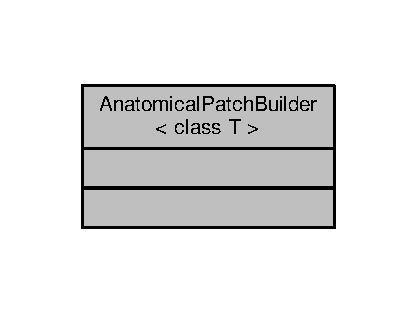
\includegraphics[width=200pt]{classAnatomicalPatchBuilder_3_01class_01T_01_4__coll__graph}
\end{center}
\end{figure}


The documentation for this class was generated from the following file\-:\begin{DoxyCompactItemize}
\item 
\hyperlink{AnatomicalPatchBuilder_8h}{Anatomical\-Patch\-Builder.\-h}\end{DoxyCompactItemize}

\hypertarget{classClinicalFrame}{\section{Clinical\-Frame Class Reference}
\label{classClinicalFrame}\index{Clinical\-Frame@{Clinical\-Frame}}
}


{\ttfamily \#include $<$Clinical\-Frame.\-h$>$}



Collaboration diagram for Clinical\-Frame\-:
\nopagebreak
\begin{figure}[H]
\begin{center}
\leavevmode
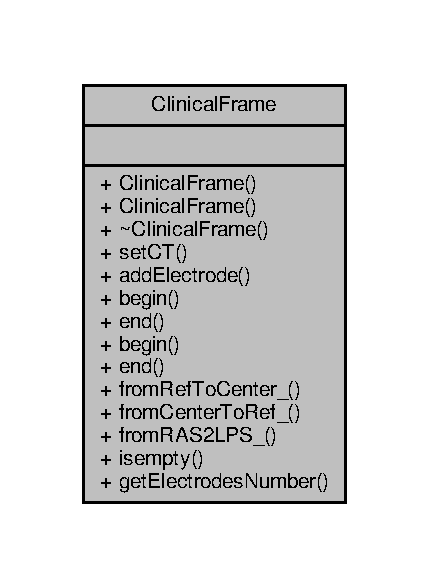
\includegraphics[width=206pt]{classClinicalFrame__coll__graph}
\end{center}
\end{figure}
\subsection*{Public Types}
\begin{DoxyCompactItemize}
\item 
typedef vector$<$ \hyperlink{classElectrode}{Electrode} $>$\\*
\-::iterator \hyperlink{classClinicalFrame_a22b67ee42a429de47c1c12ffedf1a803}{Electrode\-Iterator}
\item 
typedef vector$<$ \hyperlink{classElectrode}{Electrode} $>$\\*
\-::const\-\_\-iterator \hyperlink{classClinicalFrame_ab741d0da22f344965de240de63c8a381}{Const\-Electrode\-Iterator}
\end{DoxyCompactItemize}
\subsection*{Public Member Functions}
\begin{DoxyCompactItemize}
\item 
\hyperlink{classClinicalFrame_a63046bc9f1c3c07ea610f2761c83719a}{Clinical\-Frame} (T\-C\-L\-A\-P\-::\-Cmd\-Line $\ast$)
\item 
\hyperlink{classClinicalFrame_a213db09308126a5631c2caef5a3c21a4}{Clinical\-Frame} (void)
\item 
\hyperlink{classClinicalFrame_a3bcff6abc229e1693ae6393ca0377c27}{$\sim$\-Clinical\-Frame} (void)
\item 
void \hyperlink{classClinicalFrame_a7feb4447a4bba0aea5c6581eb3b30e82}{set\-C\-T} (\hyperlink{Definitions_8h_a6952b2a622249cc460a5875f2a793e61}{Image\-Pointer\-Type} ct)
\item 
void \hyperlink{classClinicalFrame_ac18288df5d668d1c2d39ceb1434b0076}{add\-Electrode} (\hyperlink{classElectrode}{Electrode} e)
\item 
\hyperlink{classClinicalFrame_a22b67ee42a429de47c1c12ffedf1a803}{Electrode\-Iterator} \hyperlink{classClinicalFrame_a7b3bdd254b65b20a15483c3fd91dc8de}{begin} ()
\item 
\hyperlink{classClinicalFrame_a22b67ee42a429de47c1c12ffedf1a803}{Electrode\-Iterator} \hyperlink{classClinicalFrame_a03b243aacb896873c20a2354bfe6c29c}{end} ()
\item 
\hyperlink{classClinicalFrame_ab741d0da22f344965de240de63c8a381}{Const\-Electrode\-Iterator} \hyperlink{classClinicalFrame_a11b80ea21454657e3dd1b0778b70df80}{begin} () const 
\item 
\hyperlink{classClinicalFrame_ab741d0da22f344965de240de63c8a381}{Const\-Electrode\-Iterator} \hyperlink{classClinicalFrame_a08380f480fa3f27c75c46f24ed8526a8}{end} () const 
\item 
void \hyperlink{classClinicalFrame_a68cc0496606299638370b19ee5c44f7b}{from\-Ref\-To\-Center\-\_\-} (\hyperlink{Definitions_8h_ab9d62e9721984f22424e47212a5ce25d}{Physical\-Point\-Type} $\ast$physical\-Point)
\item 
void \hyperlink{classClinicalFrame_a36849a62e3bc8414ec7c161007c38493}{from\-Center\-To\-Ref\-\_\-} (\hyperlink{Definitions_8h_ab9d62e9721984f22424e47212a5ce25d}{Physical\-Point\-Type} $\ast$physical\-Point)
\item 
void \hyperlink{classClinicalFrame_a80a3f86750d4818d5d4c2d7a50b4f529}{from\-R\-A\-S2\-L\-P\-S\-\_\-} (\hyperlink{Definitions_8h_ab9d62e9721984f22424e47212a5ce25d}{Physical\-Point\-Type} $\ast$physical\-Point)
\item 
bool \hyperlink{classClinicalFrame_ac94cf8c7ca13d597bcb961d95f7134cc}{isempty} (void) const 
\item 
int \hyperlink{classClinicalFrame_a9f970d38528bbb65dfac9e6fcae23263}{get\-Electrodes\-Number} (void) const 
\end{DoxyCompactItemize}


\subsection{Detailed Description}
\hyperlink{classClinicalFrame}{Clinical\-Frame} class

this class is the central object that holds the information for reconstruction and saves the reconstructed data. It has a pointer to C\-T data which constitutes the reference space ({\bfseries Ref. Space}) . Initially, as read from F\-C\-S\-V (3\-D\-Slicer format) each \hyperlink{classElectrode}{Electrode} has 2 points entry and target which are represented in a Centered Coordinate system. For this, the class provides methods to transform each point from Ref to Centered and back-\/ 

\subsection{Member Typedef Documentation}
\hypertarget{classClinicalFrame_ab741d0da22f344965de240de63c8a381}{\index{Clinical\-Frame@{Clinical\-Frame}!Const\-Electrode\-Iterator@{Const\-Electrode\-Iterator}}
\index{Const\-Electrode\-Iterator@{Const\-Electrode\-Iterator}!ClinicalFrame@{Clinical\-Frame}}
\subsubsection[{Const\-Electrode\-Iterator}]{\setlength{\rightskip}{0pt plus 5cm}typedef vector$<$ {\bf Electrode} $>$\-::const\-\_\-iterator {\bf Clinical\-Frame\-::\-Const\-Electrode\-Iterator}}}\label{classClinicalFrame_ab741d0da22f344965de240de63c8a381}
\hypertarget{classClinicalFrame_a22b67ee42a429de47c1c12ffedf1a803}{\index{Clinical\-Frame@{Clinical\-Frame}!Electrode\-Iterator@{Electrode\-Iterator}}
\index{Electrode\-Iterator@{Electrode\-Iterator}!ClinicalFrame@{Clinical\-Frame}}
\subsubsection[{Electrode\-Iterator}]{\setlength{\rightskip}{0pt plus 5cm}typedef vector$<$ {\bf Electrode} $>$\-::iterator {\bf Clinical\-Frame\-::\-Electrode\-Iterator}}}\label{classClinicalFrame_a22b67ee42a429de47c1c12ffedf1a803}


\subsection{Constructor \& Destructor Documentation}
\hypertarget{classClinicalFrame_a63046bc9f1c3c07ea610f2761c83719a}{\index{Clinical\-Frame@{Clinical\-Frame}!Clinical\-Frame@{Clinical\-Frame}}
\index{Clinical\-Frame@{Clinical\-Frame}!ClinicalFrame@{Clinical\-Frame}}
\subsubsection[{Clinical\-Frame}]{\setlength{\rightskip}{0pt plus 5cm}Clinical\-Frame\-::\-Clinical\-Frame (
\begin{DoxyParamCaption}
\item[{T\-C\-L\-A\-P\-::\-Cmd\-Line $\ast$}]{}
\end{DoxyParamCaption}
)\hspace{0.3cm}{\ttfamily [inline]}}}\label{classClinicalFrame_a63046bc9f1c3c07ea610f2761c83719a}
\hypertarget{classClinicalFrame_a213db09308126a5631c2caef5a3c21a4}{\index{Clinical\-Frame@{Clinical\-Frame}!Clinical\-Frame@{Clinical\-Frame}}
\index{Clinical\-Frame@{Clinical\-Frame}!ClinicalFrame@{Clinical\-Frame}}
\subsubsection[{Clinical\-Frame}]{\setlength{\rightskip}{0pt plus 5cm}Clinical\-Frame\-::\-Clinical\-Frame (
\begin{DoxyParamCaption}
\item[{void}]{}
\end{DoxyParamCaption}
)\hspace{0.3cm}{\ttfamily [inline]}}}\label{classClinicalFrame_a213db09308126a5631c2caef5a3c21a4}
\hypertarget{classClinicalFrame_a3bcff6abc229e1693ae6393ca0377c27}{\index{Clinical\-Frame@{Clinical\-Frame}!$\sim$\-Clinical\-Frame@{$\sim$\-Clinical\-Frame}}
\index{$\sim$\-Clinical\-Frame@{$\sim$\-Clinical\-Frame}!ClinicalFrame@{Clinical\-Frame}}
\subsubsection[{$\sim$\-Clinical\-Frame}]{\setlength{\rightskip}{0pt plus 5cm}Clinical\-Frame\-::$\sim$\-Clinical\-Frame (
\begin{DoxyParamCaption}
\item[{void}]{}
\end{DoxyParamCaption}
)\hspace{0.3cm}{\ttfamily [inline]}}}\label{classClinicalFrame_a3bcff6abc229e1693ae6393ca0377c27}


\subsection{Member Function Documentation}
\hypertarget{classClinicalFrame_ac18288df5d668d1c2d39ceb1434b0076}{\index{Clinical\-Frame@{Clinical\-Frame}!add\-Electrode@{add\-Electrode}}
\index{add\-Electrode@{add\-Electrode}!ClinicalFrame@{Clinical\-Frame}}
\subsubsection[{add\-Electrode}]{\setlength{\rightskip}{0pt plus 5cm}void Clinical\-Frame\-::add\-Electrode (
\begin{DoxyParamCaption}
\item[{{\bf Electrode}}]{e}
\end{DoxyParamCaption}
)\hspace{0.3cm}{\ttfamily [inline]}}}\label{classClinicalFrame_ac18288df5d668d1c2d39ceb1434b0076}
\hypertarget{classClinicalFrame_a7b3bdd254b65b20a15483c3fd91dc8de}{\index{Clinical\-Frame@{Clinical\-Frame}!begin@{begin}}
\index{begin@{begin}!ClinicalFrame@{Clinical\-Frame}}
\subsubsection[{begin}]{\setlength{\rightskip}{0pt plus 5cm}{\bf Electrode\-Iterator} Clinical\-Frame\-::begin (
\begin{DoxyParamCaption}
\item[{void}]{}
\end{DoxyParamCaption}
)\hspace{0.3cm}{\ttfamily [inline]}}}\label{classClinicalFrame_a7b3bdd254b65b20a15483c3fd91dc8de}
this function returns a pointer to H\-E\-A\-D in vector$<$ Electrode $>$ \hypertarget{classClinicalFrame_a11b80ea21454657e3dd1b0778b70df80}{\index{Clinical\-Frame@{Clinical\-Frame}!begin@{begin}}
\index{begin@{begin}!ClinicalFrame@{Clinical\-Frame}}
\subsubsection[{begin}]{\setlength{\rightskip}{0pt plus 5cm}{\bf Const\-Electrode\-Iterator} Clinical\-Frame\-::begin (
\begin{DoxyParamCaption}
\item[{void}]{}
\end{DoxyParamCaption}
) const\hspace{0.3cm}{\ttfamily [inline]}}}\label{classClinicalFrame_a11b80ea21454657e3dd1b0778b70df80}
this function returns a const pointer to H\-E\-A\-D in vector$<$ Electrode $>$ \hypertarget{classClinicalFrame_a03b243aacb896873c20a2354bfe6c29c}{\index{Clinical\-Frame@{Clinical\-Frame}!end@{end}}
\index{end@{end}!ClinicalFrame@{Clinical\-Frame}}
\subsubsection[{end}]{\setlength{\rightskip}{0pt plus 5cm}{\bf Electrode\-Iterator} Clinical\-Frame\-::end (
\begin{DoxyParamCaption}
\item[{void}]{}
\end{DoxyParamCaption}
)\hspace{0.3cm}{\ttfamily [inline]}}}\label{classClinicalFrame_a03b243aacb896873c20a2354bfe6c29c}
this function returns a pointer to T\-A\-I\-L in vector$<$ Electrode $>$ \hypertarget{classClinicalFrame_a08380f480fa3f27c75c46f24ed8526a8}{\index{Clinical\-Frame@{Clinical\-Frame}!end@{end}}
\index{end@{end}!ClinicalFrame@{Clinical\-Frame}}
\subsubsection[{end}]{\setlength{\rightskip}{0pt plus 5cm}{\bf Const\-Electrode\-Iterator} Clinical\-Frame\-::end (
\begin{DoxyParamCaption}
\item[{void}]{}
\end{DoxyParamCaption}
) const\hspace{0.3cm}{\ttfamily [inline]}}}\label{classClinicalFrame_a08380f480fa3f27c75c46f24ed8526a8}
this function returns a const pointer to T\-A\-I\-L in vector$<$ Electrode $>$ \hypertarget{classClinicalFrame_a36849a62e3bc8414ec7c161007c38493}{\index{Clinical\-Frame@{Clinical\-Frame}!from\-Center\-To\-Ref\-\_\-@{from\-Center\-To\-Ref\-\_\-}}
\index{from\-Center\-To\-Ref\-\_\-@{from\-Center\-To\-Ref\-\_\-}!ClinicalFrame@{Clinical\-Frame}}
\subsubsection[{from\-Center\-To\-Ref\-\_\-}]{\setlength{\rightskip}{0pt plus 5cm}void Clinical\-Frame\-::from\-Center\-To\-Ref\-\_\- (
\begin{DoxyParamCaption}
\item[{{\bf Physical\-Point\-Type} $\ast$}]{physical\-Point}
\end{DoxyParamCaption}
)}}\label{classClinicalFrame_a36849a62e3bc8414ec7c161007c38493}
this function transform a physical\-Point from Centered to Reference space \hypertarget{classClinicalFrame_a80a3f86750d4818d5d4c2d7a50b4f529}{\index{Clinical\-Frame@{Clinical\-Frame}!from\-R\-A\-S2\-L\-P\-S\-\_\-@{from\-R\-A\-S2\-L\-P\-S\-\_\-}}
\index{from\-R\-A\-S2\-L\-P\-S\-\_\-@{from\-R\-A\-S2\-L\-P\-S\-\_\-}!ClinicalFrame@{Clinical\-Frame}}
\subsubsection[{from\-R\-A\-S2\-L\-P\-S\-\_\-}]{\setlength{\rightskip}{0pt plus 5cm}void Clinical\-Frame\-::from\-R\-A\-S2\-L\-P\-S\-\_\- (
\begin{DoxyParamCaption}
\item[{{\bf Physical\-Point\-Type} $\ast$}]{physical\-Point}
\end{DoxyParamCaption}
)}}\label{classClinicalFrame_a80a3f86750d4818d5d4c2d7a50b4f529}
this function transform a physical\-Point from L\-P\-S to R\-A\-S space \hypertarget{classClinicalFrame_a68cc0496606299638370b19ee5c44f7b}{\index{Clinical\-Frame@{Clinical\-Frame}!from\-Ref\-To\-Center\-\_\-@{from\-Ref\-To\-Center\-\_\-}}
\index{from\-Ref\-To\-Center\-\_\-@{from\-Ref\-To\-Center\-\_\-}!ClinicalFrame@{Clinical\-Frame}}
\subsubsection[{from\-Ref\-To\-Center\-\_\-}]{\setlength{\rightskip}{0pt plus 5cm}void Clinical\-Frame\-::from\-Ref\-To\-Center\-\_\- (
\begin{DoxyParamCaption}
\item[{{\bf Physical\-Point\-Type} $\ast$}]{physical\-Point}
\end{DoxyParamCaption}
)}}\label{classClinicalFrame_a68cc0496606299638370b19ee5c44f7b}
this function transform a physical\-Point from Ref to Centered space \hypertarget{classClinicalFrame_a9f970d38528bbb65dfac9e6fcae23263}{\index{Clinical\-Frame@{Clinical\-Frame}!get\-Electrodes\-Number@{get\-Electrodes\-Number}}
\index{get\-Electrodes\-Number@{get\-Electrodes\-Number}!ClinicalFrame@{Clinical\-Frame}}
\subsubsection[{get\-Electrodes\-Number}]{\setlength{\rightskip}{0pt plus 5cm}int Clinical\-Frame\-::get\-Electrodes\-Number (
\begin{DoxyParamCaption}
\item[{void}]{}
\end{DoxyParamCaption}
) const\hspace{0.3cm}{\ttfamily [inline]}}}\label{classClinicalFrame_a9f970d38528bbb65dfac9e6fcae23263}
\hypertarget{classClinicalFrame_ac94cf8c7ca13d597bcb961d95f7134cc}{\index{Clinical\-Frame@{Clinical\-Frame}!isempty@{isempty}}
\index{isempty@{isempty}!ClinicalFrame@{Clinical\-Frame}}
\subsubsection[{isempty}]{\setlength{\rightskip}{0pt plus 5cm}bool Clinical\-Frame\-::isempty (
\begin{DoxyParamCaption}
\item[{void}]{}
\end{DoxyParamCaption}
) const\hspace{0.3cm}{\ttfamily [inline]}}}\label{classClinicalFrame_ac94cf8c7ca13d597bcb961d95f7134cc}
this function returns true or false whether the vector$<$ Electrode$>$ is empty or not \hypertarget{classClinicalFrame_a7feb4447a4bba0aea5c6581eb3b30e82}{\index{Clinical\-Frame@{Clinical\-Frame}!set\-C\-T@{set\-C\-T}}
\index{set\-C\-T@{set\-C\-T}!ClinicalFrame@{Clinical\-Frame}}
\subsubsection[{set\-C\-T}]{\setlength{\rightskip}{0pt plus 5cm}void Clinical\-Frame\-::set\-C\-T (
\begin{DoxyParamCaption}
\item[{{\bf Image\-Pointer\-Type}}]{ct}
\end{DoxyParamCaption}
)\hspace{0.3cm}{\ttfamily [inline]}}}\label{classClinicalFrame_a7feb4447a4bba0aea5c6581eb3b30e82}


The documentation for this class was generated from the following file\-:\begin{DoxyCompactItemize}
\item 
\hyperlink{ClinicalFrame_8h}{Clinical\-Frame.\-h}\end{DoxyCompactItemize}

\hypertarget{classContactConstructor}{\section{Contact\-Constructor Class Reference}
\label{classContactConstructor}\index{Contact\-Constructor@{Contact\-Constructor}}
}


{\ttfamily \#include $<$Contact\-Constructor.\-h$>$}



Collaboration diagram for Contact\-Constructor\-:
\nopagebreak
\begin{figure}[H]
\begin{center}
\leavevmode
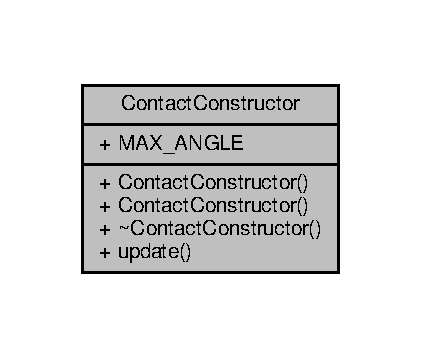
\includegraphics[width=202pt]{classContactConstructor__coll__graph}
\end{center}
\end{figure}
\subsection*{Public Member Functions}
\begin{DoxyCompactItemize}
\item 
\hyperlink{classContactConstructor_af9c80081fce365e37e2a7586b7d5ffb9}{Contact\-Constructor} (Image\-Type\-::\-Pointer ct\-Image, \hyperlink{classClinicalFrame}{Clinical\-Frame} $\ast$head\-Frame, T\-C\-L\-A\-P\-::\-Cmd\-Line $\ast$c)
\item 
\hyperlink{classContactConstructor_a0cfd4cbb2ac1c5e0583c6afadb9cdb2d}{Contact\-Constructor} (Image\-Type\-::\-Pointer ct\-Image, \hyperlink{classClinicalFrame}{Clinical\-Frame} $\ast$head\-Frame)
\item 
\hyperlink{classContactConstructor_a0e6112e4fa828e26fbca30bb577c828b}{$\sim$\-Contact\-Constructor} ()
\item 
void \hyperlink{classContactConstructor_a75bc343f91d250464589258271905bc6}{update} (void)
\end{DoxyCompactItemize}
\subsection*{Static Public Attributes}
\begin{DoxyCompactItemize}
\item 
static const double \hyperlink{classContactConstructor_af67d5c64a244708608f8736cbfd19673}{M\-A\-X\-\_\-\-A\-N\-G\-L\-E} = 0.\-988
\end{DoxyCompactItemize}


\subsection{Constructor \& Destructor Documentation}
\hypertarget{classContactConstructor_af9c80081fce365e37e2a7586b7d5ffb9}{\index{Contact\-Constructor@{Contact\-Constructor}!Contact\-Constructor@{Contact\-Constructor}}
\index{Contact\-Constructor@{Contact\-Constructor}!ContactConstructor@{Contact\-Constructor}}
\subsubsection[{Contact\-Constructor}]{\setlength{\rightskip}{0pt plus 5cm}Contact\-Constructor\-::\-Contact\-Constructor (
\begin{DoxyParamCaption}
\item[{Image\-Type\-::\-Pointer}]{ct\-Image, }
\item[{{\bf Clinical\-Frame} $\ast$}]{head\-Frame, }
\item[{T\-C\-L\-A\-P\-::\-Cmd\-Line $\ast$}]{c}
\end{DoxyParamCaption}
)\hspace{0.3cm}{\ttfamily [inline]}}}\label{classContactConstructor_af9c80081fce365e37e2a7586b7d5ffb9}
\hypertarget{classContactConstructor_a0cfd4cbb2ac1c5e0583c6afadb9cdb2d}{\index{Contact\-Constructor@{Contact\-Constructor}!Contact\-Constructor@{Contact\-Constructor}}
\index{Contact\-Constructor@{Contact\-Constructor}!ContactConstructor@{Contact\-Constructor}}
\subsubsection[{Contact\-Constructor}]{\setlength{\rightskip}{0pt plus 5cm}Contact\-Constructor\-::\-Contact\-Constructor (
\begin{DoxyParamCaption}
\item[{Image\-Type\-::\-Pointer}]{ct\-Image, }
\item[{{\bf Clinical\-Frame} $\ast$}]{head\-Frame}
\end{DoxyParamCaption}
)\hspace{0.3cm}{\ttfamily [inline]}}}\label{classContactConstructor_a0cfd4cbb2ac1c5e0583c6afadb9cdb2d}
\hypertarget{classContactConstructor_a0e6112e4fa828e26fbca30bb577c828b}{\index{Contact\-Constructor@{Contact\-Constructor}!$\sim$\-Contact\-Constructor@{$\sim$\-Contact\-Constructor}}
\index{$\sim$\-Contact\-Constructor@{$\sim$\-Contact\-Constructor}!ContactConstructor@{Contact\-Constructor}}
\subsubsection[{$\sim$\-Contact\-Constructor}]{\setlength{\rightskip}{0pt plus 5cm}Contact\-Constructor\-::$\sim$\-Contact\-Constructor (
\begin{DoxyParamCaption}
{}
\end{DoxyParamCaption}
)\hspace{0.3cm}{\ttfamily [inline]}}}\label{classContactConstructor_a0e6112e4fa828e26fbca30bb577c828b}


\subsection{Member Function Documentation}
\hypertarget{classContactConstructor_a75bc343f91d250464589258271905bc6}{\index{Contact\-Constructor@{Contact\-Constructor}!update@{update}}
\index{update@{update}!ContactConstructor@{Contact\-Constructor}}
\subsubsection[{update}]{\setlength{\rightskip}{0pt plus 5cm}void Contact\-Constructor\-::update (
\begin{DoxyParamCaption}
\item[{void}]{}
\end{DoxyParamCaption}
)}}\label{classContactConstructor_a75bc343f91d250464589258271905bc6}


\subsection{Member Data Documentation}
\hypertarget{classContactConstructor_af67d5c64a244708608f8736cbfd19673}{\index{Contact\-Constructor@{Contact\-Constructor}!M\-A\-X\-\_\-\-A\-N\-G\-L\-E@{M\-A\-X\-\_\-\-A\-N\-G\-L\-E}}
\index{M\-A\-X\-\_\-\-A\-N\-G\-L\-E@{M\-A\-X\-\_\-\-A\-N\-G\-L\-E}!ContactConstructor@{Contact\-Constructor}}
\subsubsection[{M\-A\-X\-\_\-\-A\-N\-G\-L\-E}]{\setlength{\rightskip}{0pt plus 5cm}const double Contact\-Constructor\-::\-M\-A\-X\-\_\-\-A\-N\-G\-L\-E = 0.\-988\hspace{0.3cm}{\ttfamily [static]}}}\label{classContactConstructor_af67d5c64a244708608f8736cbfd19673}


The documentation for this class was generated from the following file\-:\begin{DoxyCompactItemize}
\item 
\hyperlink{ContactConstructor_8h}{Contact\-Constructor.\-h}\end{DoxyCompactItemize}

\hypertarget{classElectrode}{\section{Electrode Class Reference}
\label{classElectrode}\index{Electrode@{Electrode}}
}


{\ttfamily \#include $<$Electrode.\-h$>$}



Collaboration diagram for Electrode\-:
\nopagebreak
\begin{figure}[H]
\begin{center}
\leavevmode
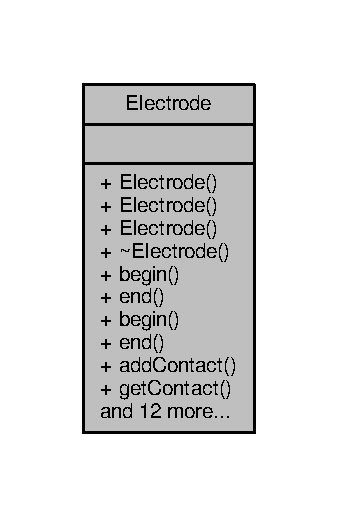
\includegraphics[width=162pt]{classElectrode__coll__graph}
\end{center}
\end{figure}
\subsection*{Public Types}
\begin{DoxyCompactItemize}
\item 
typedef \hyperlink{Definitions_8h_ab9d62e9721984f22424e47212a5ce25d}{Physical\-Point\-Type} \hyperlink{classElectrode_ac64c4a90469345a5d3e260da59765a76}{Contact}
\item 
typedef const \hyperlink{Definitions_8h_ab9d62e9721984f22424e47212a5ce25d}{Physical\-Point\-Type} \hyperlink{classElectrode_a6dc621793b4ffa70e6bc3f2627ec8bf6}{Const\-Contact}
\item 
typedef vector$<$ \hyperlink{classElectrode_ac64c4a90469345a5d3e260da59765a76}{Contact} $>$\-::iterator \hyperlink{classElectrode_a682d94c6e93fc27e2135d3a894fe9722}{Contact\-Iterator}
\item 
typedef vector$<$ \hyperlink{classElectrode_ac64c4a90469345a5d3e260da59765a76}{Contact} $>$\\*
\-::const\-\_\-iterator \hyperlink{classElectrode_a8c56b50a83beed1bf104d079083386b5}{Const\-Contact\-Iterator}
\end{DoxyCompactItemize}
\subsection*{Public Member Functions}
\begin{DoxyCompactItemize}
\item 
\hyperlink{classElectrode_a771e572c858046f109f73ee04d78e509}{Electrode} (string name, \hyperlink{classElectrode_ac64c4a90469345a5d3e260da59765a76}{Contact} \&target, \hyperlink{classElectrode_ac64c4a90469345a5d3e260da59765a76}{Contact} \&entry, T\-C\-L\-A\-P\-::\-Cmd\-Line $\ast$c)
\item 
\hyperlink{classElectrode_a3914606286820a309e87b47a79792fc8}{Electrode} (string name, \hyperlink{classElectrode_ac64c4a90469345a5d3e260da59765a76}{Contact} \&target, \hyperlink{classElectrode_ac64c4a90469345a5d3e260da59765a76}{Contact} \&entry)
\item 
\hyperlink{classElectrode_ad16409e5fbe3dbdc0d4bcfd6a148ad40}{Electrode} (string id, \hyperlink{classElectrode_ac64c4a90469345a5d3e260da59765a76}{Contact} \&target, \hyperlink{classElectrode_ac64c4a90469345a5d3e260da59765a76}{Contact} \&entry, \hyperlink{classElectrodeModel}{Electrode\-Model} m)
\item 
\hyperlink{classElectrode_aaea00b81726c5cad6a390659870ead58}{$\sim$\-Electrode} ()
\item 
\hyperlink{classElectrode_a682d94c6e93fc27e2135d3a894fe9722}{Contact\-Iterator} \hyperlink{classElectrode_a105771c0b9c630f3da68c9f220d62470}{begin} ()
\item 
\hyperlink{classElectrode_a682d94c6e93fc27e2135d3a894fe9722}{Contact\-Iterator} \hyperlink{classElectrode_ae02470004771e62d2cb9227ad2ebb6b7}{end} ()
\item 
\hyperlink{classElectrode_a8c56b50a83beed1bf104d079083386b5}{Const\-Contact\-Iterator} \hyperlink{classElectrode_af424b68151e09051b9e50cb1e087ad1d}{begin} () const 
\item 
\hyperlink{classElectrode_a8c56b50a83beed1bf104d079083386b5}{Const\-Contact\-Iterator} \hyperlink{classElectrode_a9fa4b4f90a58bc2ef4ef00bc2e8a7cbe}{end} () const 
\item 
void \hyperlink{classElectrode_a0422c73e1a10045d2efb36a96f8b48f3}{add\-Contact} (\hyperlink{classElectrode_ac64c4a90469345a5d3e260da59765a76}{Contact} c)
\item 
\hyperlink{classElectrode_a6dc621793b4ffa70e6bc3f2627ec8bf6}{Const\-Contact} $\ast$ \hyperlink{classElectrode_a3bb7efc38bbb2322722320fa5dfb14b7}{get\-Contact} (ulong id) const 
\item 
\hyperlink{classElectrode_ac64c4a90469345a5d3e260da59765a76}{Contact} $\ast$ \hyperlink{classElectrode_a16095d3177a018d40cca9e13064c69ee}{get\-Contact} (ulong id)
\item 
ulong \hyperlink{classElectrode_af9d256a3bca0873bf10177ed7acc8158}{get\-Contact\-Number} () const 
\item 
\hyperlink{classElectrode_ac64c4a90469345a5d3e260da59765a76}{Contact} \hyperlink{classElectrode_ae00ce79f47c986adedfdc34de26a4956}{get\-Target} () const 
\item 
\hyperlink{classElectrode_ac64c4a90469345a5d3e260da59765a76}{Contact} \hyperlink{classElectrode_a63534a9fcf275e30a3897bc6d5c6daec}{get\-Entry} () const 
\item 
void \hyperlink{classElectrode_a7d1686e3aaf200d8eeacd5ba5ca9b8f6}{get\-Target\-As\-Double} (double $\ast$t) const 
\item 
void \hyperlink{classElectrode_a63b949ff99a7c5a25ee2a1615231d2da}{get\-Entry\-As\-Double} (double $\ast$e) const 
\item 
void \hyperlink{classElectrode_ae1db2afe30ebad7c71a04a0c4f39b326}{set\-Target} (\hyperlink{classElectrode_ac64c4a90469345a5d3e260da59765a76}{Contact} c)
\item 
void \hyperlink{classElectrode_a2092b73cb83d1d54ff3a55a0095ffdac}{set\-Entry} (\hyperlink{classElectrode_ac64c4a90469345a5d3e260da59765a76}{Contact} c)
\item 
string \hyperlink{classElectrode_a19fa13d91444e67dbdc17891829633a2}{get\-Name} () const 
\item 
void \hyperlink{classElectrode_aac0591afceba95e538b134daad423db4}{set\-Name} (string name)
\item 
void \hyperlink{classElectrode_afe109f0f82873f28d93fc5b6f485de45}{set\-Model} (\hyperlink{classElectrodeModel}{Electrode\-Model} model)
\item 
\hyperlink{classElectrodeModel}{Electrode\-Model} \hyperlink{classElectrode_aa7d23c92c952ec3c4565be8924a8be00}{get\-Model} ()
\end{DoxyCompactItemize}
\subsection*{Friends}
\begin{DoxyCompactItemize}
\item 
ostream \& \hyperlink{classElectrode_a7ffb9f309faaf4072bda7912a86b31f4}{operator$<$$<$} (ostream \&os, const \hyperlink{classElectrode}{Electrode} \&obj)
\end{DoxyCompactItemize}


\subsection{Detailed Description}
This class represents the electrode structure 

\subsection{Member Typedef Documentation}
\hypertarget{classElectrode_a6dc621793b4ffa70e6bc3f2627ec8bf6}{\index{Electrode@{Electrode}!Const\-Contact@{Const\-Contact}}
\index{Const\-Contact@{Const\-Contact}!Electrode@{Electrode}}
\subsubsection[{Const\-Contact}]{\setlength{\rightskip}{0pt plus 5cm}typedef const {\bf Physical\-Point\-Type} {\bf Electrode\-::\-Const\-Contact}}}\label{classElectrode_a6dc621793b4ffa70e6bc3f2627ec8bf6}
\hypertarget{classElectrode_a8c56b50a83beed1bf104d079083386b5}{\index{Electrode@{Electrode}!Const\-Contact\-Iterator@{Const\-Contact\-Iterator}}
\index{Const\-Contact\-Iterator@{Const\-Contact\-Iterator}!Electrode@{Electrode}}
\subsubsection[{Const\-Contact\-Iterator}]{\setlength{\rightskip}{0pt plus 5cm}typedef vector$<$ {\bf Contact} $>$\-::const\-\_\-iterator {\bf Electrode\-::\-Const\-Contact\-Iterator}}}\label{classElectrode_a8c56b50a83beed1bf104d079083386b5}
\hypertarget{classElectrode_ac64c4a90469345a5d3e260da59765a76}{\index{Electrode@{Electrode}!Contact@{Contact}}
\index{Contact@{Contact}!Electrode@{Electrode}}
\subsubsection[{Contact}]{\setlength{\rightskip}{0pt plus 5cm}typedef {\bf Physical\-Point\-Type} {\bf Electrode\-::\-Contact}}}\label{classElectrode_ac64c4a90469345a5d3e260da59765a76}
\hypertarget{classElectrode_a682d94c6e93fc27e2135d3a894fe9722}{\index{Electrode@{Electrode}!Contact\-Iterator@{Contact\-Iterator}}
\index{Contact\-Iterator@{Contact\-Iterator}!Electrode@{Electrode}}
\subsubsection[{Contact\-Iterator}]{\setlength{\rightskip}{0pt plus 5cm}typedef vector$<$ {\bf Contact} $>$\-::iterator {\bf Electrode\-::\-Contact\-Iterator}}}\label{classElectrode_a682d94c6e93fc27e2135d3a894fe9722}


\subsection{Constructor \& Destructor Documentation}
\hypertarget{classElectrode_a771e572c858046f109f73ee04d78e509}{\index{Electrode@{Electrode}!Electrode@{Electrode}}
\index{Electrode@{Electrode}!Electrode@{Electrode}}
\subsubsection[{Electrode}]{\setlength{\rightskip}{0pt plus 5cm}Electrode\-::\-Electrode (
\begin{DoxyParamCaption}
\item[{string}]{name, }
\item[{{\bf Contact} \&}]{target, }
\item[{{\bf Contact} \&}]{entry, }
\item[{T\-C\-L\-A\-P\-::\-Cmd\-Line $\ast$}]{c}
\end{DoxyParamCaption}
)\hspace{0.3cm}{\ttfamily [inline]}}}\label{classElectrode_a771e572c858046f109f73ee04d78e509}
\hypertarget{classElectrode_a3914606286820a309e87b47a79792fc8}{\index{Electrode@{Electrode}!Electrode@{Electrode}}
\index{Electrode@{Electrode}!Electrode@{Electrode}}
\subsubsection[{Electrode}]{\setlength{\rightskip}{0pt plus 5cm}Electrode\-::\-Electrode (
\begin{DoxyParamCaption}
\item[{string}]{name, }
\item[{{\bf Contact} \&}]{target, }
\item[{{\bf Contact} \&}]{entry}
\end{DoxyParamCaption}
)\hspace{0.3cm}{\ttfamily [inline]}}}\label{classElectrode_a3914606286820a309e87b47a79792fc8}
\hypertarget{classElectrode_ad16409e5fbe3dbdc0d4bcfd6a148ad40}{\index{Electrode@{Electrode}!Electrode@{Electrode}}
\index{Electrode@{Electrode}!Electrode@{Electrode}}
\subsubsection[{Electrode}]{\setlength{\rightskip}{0pt plus 5cm}Electrode\-::\-Electrode (
\begin{DoxyParamCaption}
\item[{string}]{id, }
\item[{{\bf Contact} \&}]{target, }
\item[{{\bf Contact} \&}]{entry, }
\item[{{\bf Electrode\-Model}}]{m}
\end{DoxyParamCaption}
)}}\label{classElectrode_ad16409e5fbe3dbdc0d4bcfd6a148ad40}
\hypertarget{classElectrode_aaea00b81726c5cad6a390659870ead58}{\index{Electrode@{Electrode}!$\sim$\-Electrode@{$\sim$\-Electrode}}
\index{$\sim$\-Electrode@{$\sim$\-Electrode}!Electrode@{Electrode}}
\subsubsection[{$\sim$\-Electrode}]{\setlength{\rightskip}{0pt plus 5cm}Electrode\-::$\sim$\-Electrode (
\begin{DoxyParamCaption}
{}
\end{DoxyParamCaption}
)\hspace{0.3cm}{\ttfamily [inline]}}}\label{classElectrode_aaea00b81726c5cad6a390659870ead58}


\subsection{Member Function Documentation}
\hypertarget{classElectrode_a0422c73e1a10045d2efb36a96f8b48f3}{\index{Electrode@{Electrode}!add\-Contact@{add\-Contact}}
\index{add\-Contact@{add\-Contact}!Electrode@{Electrode}}
\subsubsection[{add\-Contact}]{\setlength{\rightskip}{0pt plus 5cm}void Electrode\-::add\-Contact (
\begin{DoxyParamCaption}
\item[{{\bf Contact}}]{c}
\end{DoxyParamCaption}
)\hspace{0.3cm}{\ttfamily [inline]}}}\label{classElectrode_a0422c73e1a10045d2efb36a96f8b48f3}
\hypertarget{classElectrode_a105771c0b9c630f3da68c9f220d62470}{\index{Electrode@{Electrode}!begin@{begin}}
\index{begin@{begin}!Electrode@{Electrode}}
\subsubsection[{begin}]{\setlength{\rightskip}{0pt plus 5cm}{\bf Contact\-Iterator} Electrode\-::begin (
\begin{DoxyParamCaption}
\item[{void}]{}
\end{DoxyParamCaption}
)\hspace{0.3cm}{\ttfamily [inline]}}}\label{classElectrode_a105771c0b9c630f3da68c9f220d62470}
this method returns a pointer to H\-E\-A\-D of vector$<$ Contact $>$ \hypertarget{classElectrode_af424b68151e09051b9e50cb1e087ad1d}{\index{Electrode@{Electrode}!begin@{begin}}
\index{begin@{begin}!Electrode@{Electrode}}
\subsubsection[{begin}]{\setlength{\rightskip}{0pt plus 5cm}{\bf Const\-Contact\-Iterator} Electrode\-::begin (
\begin{DoxyParamCaption}
\item[{void}]{}
\end{DoxyParamCaption}
) const\hspace{0.3cm}{\ttfamily [inline]}}}\label{classElectrode_af424b68151e09051b9e50cb1e087ad1d}
this method returns a const pointer to H\-E\-A\-D of vector$<$ Contact $>$ \hypertarget{classElectrode_ae02470004771e62d2cb9227ad2ebb6b7}{\index{Electrode@{Electrode}!end@{end}}
\index{end@{end}!Electrode@{Electrode}}
\subsubsection[{end}]{\setlength{\rightskip}{0pt plus 5cm}{\bf Contact\-Iterator} Electrode\-::end (
\begin{DoxyParamCaption}
\item[{void}]{}
\end{DoxyParamCaption}
)\hspace{0.3cm}{\ttfamily [inline]}}}\label{classElectrode_ae02470004771e62d2cb9227ad2ebb6b7}
this method returns a pointer to T\-A\-I\-L of vector$<$ Contact $>$ \hypertarget{classElectrode_a9fa4b4f90a58bc2ef4ef00bc2e8a7cbe}{\index{Electrode@{Electrode}!end@{end}}
\index{end@{end}!Electrode@{Electrode}}
\subsubsection[{end}]{\setlength{\rightskip}{0pt plus 5cm}{\bf Const\-Contact\-Iterator} Electrode\-::end (
\begin{DoxyParamCaption}
\item[{void}]{}
\end{DoxyParamCaption}
) const\hspace{0.3cm}{\ttfamily [inline]}}}\label{classElectrode_a9fa4b4f90a58bc2ef4ef00bc2e8a7cbe}
this method returns a const pointer to T\-A\-I\-L of vector$<$ Contact $>$ \hypertarget{classElectrode_a3bb7efc38bbb2322722320fa5dfb14b7}{\index{Electrode@{Electrode}!get\-Contact@{get\-Contact}}
\index{get\-Contact@{get\-Contact}!Electrode@{Electrode}}
\subsubsection[{get\-Contact}]{\setlength{\rightskip}{0pt plus 5cm}{\bf Const\-Contact}$\ast$ Electrode\-::get\-Contact (
\begin{DoxyParamCaption}
\item[{ulong}]{id}
\end{DoxyParamCaption}
) const\hspace{0.3cm}{\ttfamily [inline]}}}\label{classElectrode_a3bb7efc38bbb2322722320fa5dfb14b7}
get const pointer to contact given contact position along vector $<$ Contact $>$ 
\begin{DoxyParams}{Parameters}
{\em id} & the contact index in vector \\
\hline
\end{DoxyParams}
\begin{DoxyReturn}{Returns}
N\-U\-L\-L pointer in case of overflow (id $>$ vector.\-size) 
\end{DoxyReturn}
\hypertarget{classElectrode_a16095d3177a018d40cca9e13064c69ee}{\index{Electrode@{Electrode}!get\-Contact@{get\-Contact}}
\index{get\-Contact@{get\-Contact}!Electrode@{Electrode}}
\subsubsection[{get\-Contact}]{\setlength{\rightskip}{0pt plus 5cm}{\bf Contact}$\ast$ Electrode\-::get\-Contact (
\begin{DoxyParamCaption}
\item[{ulong}]{id}
\end{DoxyParamCaption}
)\hspace{0.3cm}{\ttfamily [inline]}}}\label{classElectrode_a16095d3177a018d40cca9e13064c69ee}
get pointer to contact given contact position along vector $<$ Contact $>$ 
\begin{DoxyParams}{Parameters}
{\em id} & the contact index in vector \\
\hline
\end{DoxyParams}
\begin{DoxyReturn}{Returns}
N\-U\-L\-L pointer in case of overflow (id $>$ vector.\-size) 
\end{DoxyReturn}
\hypertarget{classElectrode_af9d256a3bca0873bf10177ed7acc8158}{\index{Electrode@{Electrode}!get\-Contact\-Number@{get\-Contact\-Number}}
\index{get\-Contact\-Number@{get\-Contact\-Number}!Electrode@{Electrode}}
\subsubsection[{get\-Contact\-Number}]{\setlength{\rightskip}{0pt plus 5cm}ulong Electrode\-::get\-Contact\-Number (
\begin{DoxyParamCaption}
{}
\end{DoxyParamCaption}
) const\hspace{0.3cm}{\ttfamily [inline]}}}\label{classElectrode_af9d256a3bca0873bf10177ed7acc8158}
get number of contacts present in vector$<$ Contact $>$ \hypertarget{classElectrode_a63534a9fcf275e30a3897bc6d5c6daec}{\index{Electrode@{Electrode}!get\-Entry@{get\-Entry}}
\index{get\-Entry@{get\-Entry}!Electrode@{Electrode}}
\subsubsection[{get\-Entry}]{\setlength{\rightskip}{0pt plus 5cm}{\bf Contact} Electrode\-::get\-Entry (
\begin{DoxyParamCaption}
{}
\end{DoxyParamCaption}
) const\hspace{0.3cm}{\ttfamily [inline]}}}\label{classElectrode_a63534a9fcf275e30a3897bc6d5c6daec}
this function returns the entry point in mm as read from fiducial list \hypertarget{classElectrode_a63b949ff99a7c5a25ee2a1615231d2da}{\index{Electrode@{Electrode}!get\-Entry\-As\-Double@{get\-Entry\-As\-Double}}
\index{get\-Entry\-As\-Double@{get\-Entry\-As\-Double}!Electrode@{Electrode}}
\subsubsection[{get\-Entry\-As\-Double}]{\setlength{\rightskip}{0pt plus 5cm}void Electrode\-::get\-Entry\-As\-Double (
\begin{DoxyParamCaption}
\item[{double $\ast$}]{e}
\end{DoxyParamCaption}
) const\hspace{0.3cm}{\ttfamily [inline]}}}\label{classElectrode_a63b949ff99a7c5a25ee2a1615231d2da}
this function converts Contact entry to double\mbox{[}3\mbox{]} entry \hypertarget{classElectrode_aa7d23c92c952ec3c4565be8924a8be00}{\index{Electrode@{Electrode}!get\-Model@{get\-Model}}
\index{get\-Model@{get\-Model}!Electrode@{Electrode}}
\subsubsection[{get\-Model}]{\setlength{\rightskip}{0pt plus 5cm}{\bf Electrode\-Model} Electrode\-::get\-Model (
\begin{DoxyParamCaption}
{}
\end{DoxyParamCaption}
)\hspace{0.3cm}{\ttfamily [inline]}}}\label{classElectrode_aa7d23c92c952ec3c4565be8924a8be00}
\hypertarget{classElectrode_a19fa13d91444e67dbdc17891829633a2}{\index{Electrode@{Electrode}!get\-Name@{get\-Name}}
\index{get\-Name@{get\-Name}!Electrode@{Electrode}}
\subsubsection[{get\-Name}]{\setlength{\rightskip}{0pt plus 5cm}string Electrode\-::get\-Name (
\begin{DoxyParamCaption}
{}
\end{DoxyParamCaption}
) const\hspace{0.3cm}{\ttfamily [inline]}}}\label{classElectrode_a19fa13d91444e67dbdc17891829633a2}
\hypertarget{classElectrode_ae00ce79f47c986adedfdc34de26a4956}{\index{Electrode@{Electrode}!get\-Target@{get\-Target}}
\index{get\-Target@{get\-Target}!Electrode@{Electrode}}
\subsubsection[{get\-Target}]{\setlength{\rightskip}{0pt plus 5cm}{\bf Contact} Electrode\-::get\-Target (
\begin{DoxyParamCaption}
{}
\end{DoxyParamCaption}
) const\hspace{0.3cm}{\ttfamily [inline]}}}\label{classElectrode_ae00ce79f47c986adedfdc34de26a4956}
this function returns the target point in mm as read from fiducial list \hypertarget{classElectrode_a7d1686e3aaf200d8eeacd5ba5ca9b8f6}{\index{Electrode@{Electrode}!get\-Target\-As\-Double@{get\-Target\-As\-Double}}
\index{get\-Target\-As\-Double@{get\-Target\-As\-Double}!Electrode@{Electrode}}
\subsubsection[{get\-Target\-As\-Double}]{\setlength{\rightskip}{0pt plus 5cm}void Electrode\-::get\-Target\-As\-Double (
\begin{DoxyParamCaption}
\item[{double $\ast$}]{t}
\end{DoxyParamCaption}
) const\hspace{0.3cm}{\ttfamily [inline]}}}\label{classElectrode_a7d1686e3aaf200d8eeacd5ba5ca9b8f6}
this function converts Contact target to double\mbox{[}3\mbox{]} target \hypertarget{classElectrode_a2092b73cb83d1d54ff3a55a0095ffdac}{\index{Electrode@{Electrode}!set\-Entry@{set\-Entry}}
\index{set\-Entry@{set\-Entry}!Electrode@{Electrode}}
\subsubsection[{set\-Entry}]{\setlength{\rightskip}{0pt plus 5cm}void Electrode\-::set\-Entry (
\begin{DoxyParamCaption}
\item[{{\bf Contact}}]{c}
\end{DoxyParamCaption}
)\hspace{0.3cm}{\ttfamily [inline]}}}\label{classElectrode_a2092b73cb83d1d54ff3a55a0095ffdac}
\hypertarget{classElectrode_afe109f0f82873f28d93fc5b6f485de45}{\index{Electrode@{Electrode}!set\-Model@{set\-Model}}
\index{set\-Model@{set\-Model}!Electrode@{Electrode}}
\subsubsection[{set\-Model}]{\setlength{\rightskip}{0pt plus 5cm}void Electrode\-::set\-Model (
\begin{DoxyParamCaption}
\item[{{\bf Electrode\-Model}}]{model}
\end{DoxyParamCaption}
)}}\label{classElectrode_afe109f0f82873f28d93fc5b6f485de45}
\hypertarget{classElectrode_aac0591afceba95e538b134daad423db4}{\index{Electrode@{Electrode}!set\-Name@{set\-Name}}
\index{set\-Name@{set\-Name}!Electrode@{Electrode}}
\subsubsection[{set\-Name}]{\setlength{\rightskip}{0pt plus 5cm}void Electrode\-::set\-Name (
\begin{DoxyParamCaption}
\item[{string}]{name}
\end{DoxyParamCaption}
)\hspace{0.3cm}{\ttfamily [inline]}}}\label{classElectrode_aac0591afceba95e538b134daad423db4}
\hypertarget{classElectrode_ae1db2afe30ebad7c71a04a0c4f39b326}{\index{Electrode@{Electrode}!set\-Target@{set\-Target}}
\index{set\-Target@{set\-Target}!Electrode@{Electrode}}
\subsubsection[{set\-Target}]{\setlength{\rightskip}{0pt plus 5cm}void Electrode\-::set\-Target (
\begin{DoxyParamCaption}
\item[{{\bf Contact}}]{c}
\end{DoxyParamCaption}
)\hspace{0.3cm}{\ttfamily [inline]}}}\label{classElectrode_ae1db2afe30ebad7c71a04a0c4f39b326}


\subsection{Friends And Related Function Documentation}
\hypertarget{classElectrode_a7ffb9f309faaf4072bda7912a86b31f4}{\index{Electrode@{Electrode}!operator$<$$<$@{operator$<$$<$}}
\index{operator$<$$<$@{operator$<$$<$}!Electrode@{Electrode}}
\subsubsection[{operator$<$$<$}]{\setlength{\rightskip}{0pt plus 5cm}ostream\& operator$<$$<$ (
\begin{DoxyParamCaption}
\item[{ostream \&}]{os, }
\item[{const {\bf Electrode} \&}]{obj}
\end{DoxyParamCaption}
)\hspace{0.3cm}{\ttfamily [friend]}}}\label{classElectrode_a7ffb9f309faaf4072bda7912a86b31f4}


The documentation for this class was generated from the following file\-:\begin{DoxyCompactItemize}
\item 
\hyperlink{Electrode_8h}{Electrode.\-h}\end{DoxyCompactItemize}

\hypertarget{classElectrodeModel}{\section{Electrode\-Model Class Reference}
\label{classElectrodeModel}\index{Electrode\-Model@{Electrode\-Model}}
}


{\ttfamily \#include $<$Electrode\-Model.\-h$>$}



Collaboration diagram for Electrode\-Model\-:
\nopagebreak
\begin{figure}[H]
\begin{center}
\leavevmode
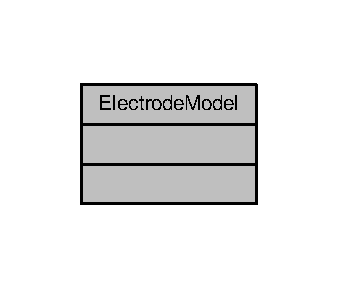
\includegraphics[width=162pt]{classElectrodeModel__coll__graph}
\end{center}
\end{figure}


The documentation for this class was generated from the following file\-:\begin{DoxyCompactItemize}
\item 
\hyperlink{ElectrodeModel_8h}{Electrode\-Model.\-h}\end{DoxyCompactItemize}

\hypertarget{classFCSVReader}{\section{F\-C\-S\-V\-Reader Class Reference}
\label{classFCSVReader}\index{F\-C\-S\-V\-Reader@{F\-C\-S\-V\-Reader}}
}


{\ttfamily \#include $<$F\-C\-S\-V\-Reader.\-h$>$}



Collaboration diagram for F\-C\-S\-V\-Reader\-:
\nopagebreak
\begin{figure}[H]
\begin{center}
\leavevmode
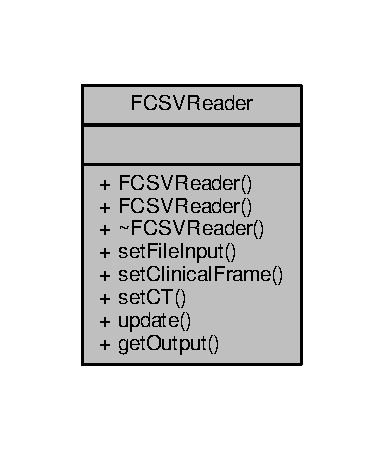
\includegraphics[width=184pt]{classFCSVReader__coll__graph}
\end{center}
\end{figure}
\subsection*{Public Member Functions}
\begin{DoxyCompactItemize}
\item 
\hyperlink{classFCSVReader_a1b2b7d8b966678d8f808bb3cbce0915b}{F\-C\-S\-V\-Reader} (T\-C\-L\-A\-P\-::\-Cmd\-Line $\ast$c)
\item 
\hyperlink{classFCSVReader_a708da1f7923ad87643797f11d15c2703}{F\-C\-S\-V\-Reader} (string $\ast$filein, T\-C\-L\-A\-P\-::\-Cmd\-Line $\ast$c)
\item 
\hyperlink{classFCSVReader_aafeed39a9516b04df7364564593c948a}{$\sim$\-F\-C\-S\-V\-Reader} ()
\item 
void \hyperlink{classFCSVReader_a47d8fde50cb1506f681fa7bbf464b816}{set\-File\-Input} (string $\ast$filein)
\item 
void \hyperlink{classFCSVReader_a1b056959e112ca1a028ce9ef880ff071}{set\-Clinical\-Frame} (\hyperlink{classClinicalFrame}{Clinical\-Frame} $\ast$cf)
\item 
void \hyperlink{classFCSVReader_ad78a979d3c97883741ad81306540ea69}{set\-C\-T} (Image\-Type\-::\-Pointer ct\-Image)
\item 
int \hyperlink{classFCSVReader_ac5654025633d18b402f0349b33765254}{update} (void)
\item 
\hyperlink{classClinicalFrame}{Clinical\-Frame} $\ast$ \hyperlink{classFCSVReader_a3cee91a10c90ce2310c241ae4fd4d85a}{get\-Output} ()
\end{DoxyCompactItemize}


\subsection{Detailed Description}
A\-S\-S\-U\-M\-E\-: C\-T is nifti, so must be R\-A\-S and Ref. for this reason we assume that the fiducial list {\itshape have} to be in R\-A\-S and Ref format.

N\-O\-T\-I\-C\-E\-: I\-T\-K\-Reader transform automatically the C\-T into L\-P\-S, so we need to do the same for the fiducial lit.

T\-O\-D\-O\-: \hyperlink{classFCSVReader}{F\-C\-S\-V\-Reader} legge il file direttamente dalla command line, per cui l'opzione di file reader e' lui che deve aggiungerla. This class reads entry and target points from fiducial file and outputs the clinical frame. this assumes that fiducial data are represented in L\-P\-S -\/ Centered space. Usually file constructed with 3\-D\-Slicer are defined in this space. 

\subsection{Constructor \& Destructor Documentation}
\hypertarget{classFCSVReader_a1b2b7d8b966678d8f808bb3cbce0915b}{\index{F\-C\-S\-V\-Reader@{F\-C\-S\-V\-Reader}!F\-C\-S\-V\-Reader@{F\-C\-S\-V\-Reader}}
\index{F\-C\-S\-V\-Reader@{F\-C\-S\-V\-Reader}!FCSVReader@{F\-C\-S\-V\-Reader}}
\subsubsection[{F\-C\-S\-V\-Reader}]{\setlength{\rightskip}{0pt plus 5cm}F\-C\-S\-V\-Reader\-::\-F\-C\-S\-V\-Reader (
\begin{DoxyParamCaption}
\item[{T\-C\-L\-A\-P\-::\-Cmd\-Line $\ast$}]{c}
\end{DoxyParamCaption}
)\hspace{0.3cm}{\ttfamily [inline]}}}\label{classFCSVReader_a1b2b7d8b966678d8f808bb3cbce0915b}
\hypertarget{classFCSVReader_a708da1f7923ad87643797f11d15c2703}{\index{F\-C\-S\-V\-Reader@{F\-C\-S\-V\-Reader}!F\-C\-S\-V\-Reader@{F\-C\-S\-V\-Reader}}
\index{F\-C\-S\-V\-Reader@{F\-C\-S\-V\-Reader}!FCSVReader@{F\-C\-S\-V\-Reader}}
\subsubsection[{F\-C\-S\-V\-Reader}]{\setlength{\rightskip}{0pt plus 5cm}F\-C\-S\-V\-Reader\-::\-F\-C\-S\-V\-Reader (
\begin{DoxyParamCaption}
\item[{string $\ast$}]{filein, }
\item[{T\-C\-L\-A\-P\-::\-Cmd\-Line $\ast$}]{c}
\end{DoxyParamCaption}
)\hspace{0.3cm}{\ttfamily [inline]}}}\label{classFCSVReader_a708da1f7923ad87643797f11d15c2703}
\hypertarget{classFCSVReader_aafeed39a9516b04df7364564593c948a}{\index{F\-C\-S\-V\-Reader@{F\-C\-S\-V\-Reader}!$\sim$\-F\-C\-S\-V\-Reader@{$\sim$\-F\-C\-S\-V\-Reader}}
\index{$\sim$\-F\-C\-S\-V\-Reader@{$\sim$\-F\-C\-S\-V\-Reader}!FCSVReader@{F\-C\-S\-V\-Reader}}
\subsubsection[{$\sim$\-F\-C\-S\-V\-Reader}]{\setlength{\rightskip}{0pt plus 5cm}F\-C\-S\-V\-Reader\-::$\sim$\-F\-C\-S\-V\-Reader (
\begin{DoxyParamCaption}
{}
\end{DoxyParamCaption}
)\hspace{0.3cm}{\ttfamily [inline]}}}\label{classFCSVReader_aafeed39a9516b04df7364564593c948a}


\subsection{Member Function Documentation}
\hypertarget{classFCSVReader_a3cee91a10c90ce2310c241ae4fd4d85a}{\index{F\-C\-S\-V\-Reader@{F\-C\-S\-V\-Reader}!get\-Output@{get\-Output}}
\index{get\-Output@{get\-Output}!FCSVReader@{F\-C\-S\-V\-Reader}}
\subsubsection[{get\-Output}]{\setlength{\rightskip}{0pt plus 5cm}{\bf Clinical\-Frame}$\ast$ F\-C\-S\-V\-Reader\-::get\-Output (
\begin{DoxyParamCaption}
{}
\end{DoxyParamCaption}
)\hspace{0.3cm}{\ttfamily [inline]}}}\label{classFCSVReader_a3cee91a10c90ce2310c241ae4fd4d85a}
returns a pointer to the constructed \hyperlink{classClinicalFrame}{Clinical\-Frame} \hypertarget{classFCSVReader_a1b056959e112ca1a028ce9ef880ff071}{\index{F\-C\-S\-V\-Reader@{F\-C\-S\-V\-Reader}!set\-Clinical\-Frame@{set\-Clinical\-Frame}}
\index{set\-Clinical\-Frame@{set\-Clinical\-Frame}!FCSVReader@{F\-C\-S\-V\-Reader}}
\subsubsection[{set\-Clinical\-Frame}]{\setlength{\rightskip}{0pt plus 5cm}void F\-C\-S\-V\-Reader\-::set\-Clinical\-Frame (
\begin{DoxyParamCaption}
\item[{{\bf Clinical\-Frame} $\ast$}]{cf}
\end{DoxyParamCaption}
)\hspace{0.3cm}{\ttfamily [inline]}}}\label{classFCSVReader_a1b056959e112ca1a028ce9ef880ff071}
\hypertarget{classFCSVReader_ad78a979d3c97883741ad81306540ea69}{\index{F\-C\-S\-V\-Reader@{F\-C\-S\-V\-Reader}!set\-C\-T@{set\-C\-T}}
\index{set\-C\-T@{set\-C\-T}!FCSVReader@{F\-C\-S\-V\-Reader}}
\subsubsection[{set\-C\-T}]{\setlength{\rightskip}{0pt plus 5cm}void F\-C\-S\-V\-Reader\-::set\-C\-T (
\begin{DoxyParamCaption}
\item[{Image\-Type\-::\-Pointer}]{ct\-Image}
\end{DoxyParamCaption}
)}}\label{classFCSVReader_ad78a979d3c97883741ad81306540ea69}
\hypertarget{classFCSVReader_a47d8fde50cb1506f681fa7bbf464b816}{\index{F\-C\-S\-V\-Reader@{F\-C\-S\-V\-Reader}!set\-File\-Input@{set\-File\-Input}}
\index{set\-File\-Input@{set\-File\-Input}!FCSVReader@{F\-C\-S\-V\-Reader}}
\subsubsection[{set\-File\-Input}]{\setlength{\rightskip}{0pt plus 5cm}void F\-C\-S\-V\-Reader\-::set\-File\-Input (
\begin{DoxyParamCaption}
\item[{string $\ast$}]{filein}
\end{DoxyParamCaption}
)\hspace{0.3cm}{\ttfamily [inline]}}}\label{classFCSVReader_a47d8fde50cb1506f681fa7bbf464b816}
\hypertarget{classFCSVReader_ac5654025633d18b402f0349b33765254}{\index{F\-C\-S\-V\-Reader@{F\-C\-S\-V\-Reader}!update@{update}}
\index{update@{update}!FCSVReader@{F\-C\-S\-V\-Reader}}
\subsubsection[{update}]{\setlength{\rightskip}{0pt plus 5cm}int F\-C\-S\-V\-Reader\-::update (
\begin{DoxyParamCaption}
\item[{void}]{}
\end{DoxyParamCaption}
)}}\label{classFCSVReader_ac5654025633d18b402f0349b33765254}
This function actually reads the fiducial file and populate the \hyperlink{classClinicalFrame}{Clinical\-Frame} information it's not important the order of entry/target points till they are represented in L\-P\-S-\/\-Centered space. This function computes the distance from the center (0,0,0) to understand whether a coordiante triplet is a target or entry point. Comments at the beginning of file are ignored. 

The documentation for this class was generated from the following file\-:\begin{DoxyCompactItemize}
\item 
\hyperlink{FCSVReader_8h}{F\-C\-S\-V\-Reader.\-h}\end{DoxyCompactItemize}

\hypertarget{classFCSVWriter}{\section{F\-C\-S\-V\-Writer Class Reference}
\label{classFCSVWriter}\index{F\-C\-S\-V\-Writer@{F\-C\-S\-V\-Writer}}
}


{\ttfamily \#include $<$F\-C\-S\-V\-Writer.\-h$>$}



Inheritance diagram for F\-C\-S\-V\-Writer\-:
\nopagebreak
\begin{figure}[H]
\begin{center}
\leavevmode
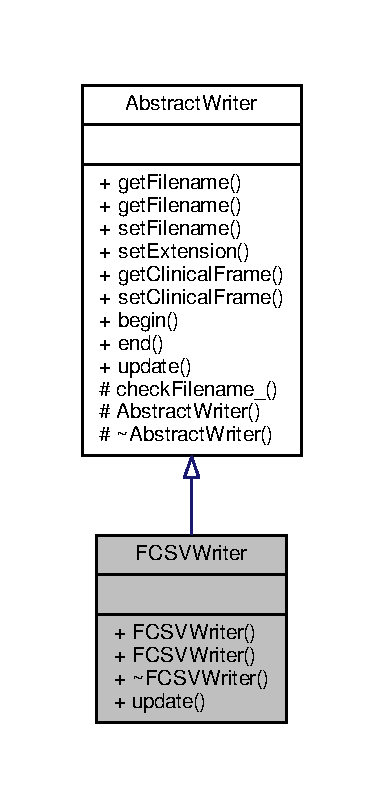
\includegraphics[width=184pt]{classFCSVWriter__inherit__graph}
\end{center}
\end{figure}


Collaboration diagram for F\-C\-S\-V\-Writer\-:
\nopagebreak
\begin{figure}[H]
\begin{center}
\leavevmode
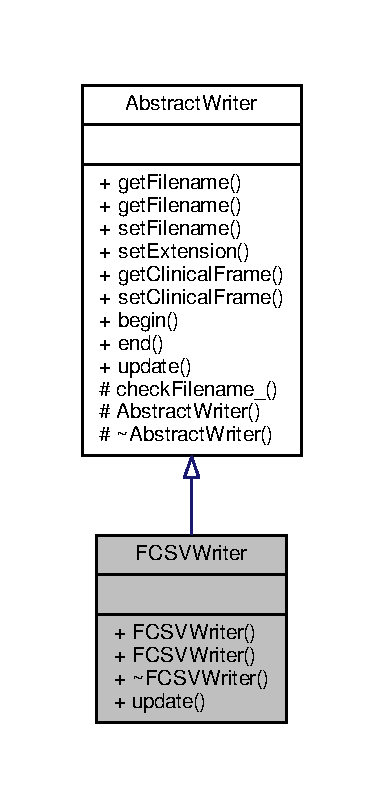
\includegraphics[width=184pt]{classFCSVWriter__coll__graph}
\end{center}
\end{figure}
\subsection*{Public Member Functions}
\begin{DoxyCompactItemize}
\item 
\hyperlink{classFCSVWriter_a149edd9e0a44bc277c00972c8f38ef79}{F\-C\-S\-V\-Writer} (string filename, T\-C\-L\-A\-P\-::\-Cmd\-Line \&cmd)
\item 
\hyperlink{classFCSVWriter_a330d506d30964c277f0b2d025e61ca26}{F\-C\-S\-V\-Writer} (string filename)
\item 
virtual \hyperlink{classFCSVWriter_aa73bd2305a61f453953ec9c2f976f10c}{$\sim$\-F\-C\-S\-V\-Writer} (void)
\item 
int \hyperlink{classFCSVWriter_a23b5071a6eda497f4ce7872c6af6ae5c}{update} ()
\end{DoxyCompactItemize}
\subsection*{Additional Inherited Members}


\subsection{Detailed Description}
\hyperlink{classFCSVWriter}{F\-C\-S\-V\-Writer} class This class implements 3\-D\-Slicer fiducial list for reconstructed data. A\-T\-M, only v3 standard is supported. v4 support (which consists in a single file for fiducial point will be handled in next stable release (since v4 support v3 std as retro-\/comp) 

\subsection{Constructor \& Destructor Documentation}
\hypertarget{classFCSVWriter_a149edd9e0a44bc277c00972c8f38ef79}{\index{F\-C\-S\-V\-Writer@{F\-C\-S\-V\-Writer}!F\-C\-S\-V\-Writer@{F\-C\-S\-V\-Writer}}
\index{F\-C\-S\-V\-Writer@{F\-C\-S\-V\-Writer}!FCSVWriter@{F\-C\-S\-V\-Writer}}
\subsubsection[{F\-C\-S\-V\-Writer}]{\setlength{\rightskip}{0pt plus 5cm}F\-C\-S\-V\-Writer\-::\-F\-C\-S\-V\-Writer (
\begin{DoxyParamCaption}
\item[{string}]{filename, }
\item[{T\-C\-L\-A\-P\-::\-Cmd\-Line \&}]{cmd}
\end{DoxyParamCaption}
)\hspace{0.3cm}{\ttfamily [inline]}}}\label{classFCSVWriter_a149edd9e0a44bc277c00972c8f38ef79}
\hypertarget{classFCSVWriter_a330d506d30964c277f0b2d025e61ca26}{\index{F\-C\-S\-V\-Writer@{F\-C\-S\-V\-Writer}!F\-C\-S\-V\-Writer@{F\-C\-S\-V\-Writer}}
\index{F\-C\-S\-V\-Writer@{F\-C\-S\-V\-Writer}!FCSVWriter@{F\-C\-S\-V\-Writer}}
\subsubsection[{F\-C\-S\-V\-Writer}]{\setlength{\rightskip}{0pt plus 5cm}F\-C\-S\-V\-Writer\-::\-F\-C\-S\-V\-Writer (
\begin{DoxyParamCaption}
\item[{string}]{filename}
\end{DoxyParamCaption}
)\hspace{0.3cm}{\ttfamily [inline]}}}\label{classFCSVWriter_a330d506d30964c277f0b2d025e61ca26}
\hypertarget{classFCSVWriter_aa73bd2305a61f453953ec9c2f976f10c}{\index{F\-C\-S\-V\-Writer@{F\-C\-S\-V\-Writer}!$\sim$\-F\-C\-S\-V\-Writer@{$\sim$\-F\-C\-S\-V\-Writer}}
\index{$\sim$\-F\-C\-S\-V\-Writer@{$\sim$\-F\-C\-S\-V\-Writer}!FCSVWriter@{F\-C\-S\-V\-Writer}}
\subsubsection[{$\sim$\-F\-C\-S\-V\-Writer}]{\setlength{\rightskip}{0pt plus 5cm}virtual F\-C\-S\-V\-Writer\-::$\sim$\-F\-C\-S\-V\-Writer (
\begin{DoxyParamCaption}
\item[{void}]{}
\end{DoxyParamCaption}
)\hspace{0.3cm}{\ttfamily [inline]}, {\ttfamily [virtual]}}}\label{classFCSVWriter_aa73bd2305a61f453953ec9c2f976f10c}


\subsection{Member Function Documentation}
\hypertarget{classFCSVWriter_a23b5071a6eda497f4ce7872c6af6ae5c}{\index{F\-C\-S\-V\-Writer@{F\-C\-S\-V\-Writer}!update@{update}}
\index{update@{update}!FCSVWriter@{F\-C\-S\-V\-Writer}}
\subsubsection[{update}]{\setlength{\rightskip}{0pt plus 5cm}int F\-C\-S\-V\-Writer\-::update (
\begin{DoxyParamCaption}
\item[{void}]{}
\end{DoxyParamCaption}
)\hspace{0.3cm}{\ttfamily [virtual]}}}\label{classFCSVWriter_a23b5071a6eda497f4ce7872c6af6ae5c}
it writes down the recontructed data 

Implements \hyperlink{classAbstractWriter_ae3d1e946840352b28b092902664a1115}{Abstract\-Writer}.



The documentation for this class was generated from the following file\-:\begin{DoxyCompactItemize}
\item 
\hyperlink{FCSVWriter_8h}{F\-C\-S\-V\-Writer.\-h}\end{DoxyCompactItemize}

\hypertarget{classGMPIEstimator}{\section{G\-M\-P\-I\-Estimator Class Reference}
\label{classGMPIEstimator}\index{G\-M\-P\-I\-Estimator@{G\-M\-P\-I\-Estimator}}
}


{\ttfamily \#include $<$G\-M\-P\-I\-Estimator.\-h$>$}



Collaboration diagram for G\-M\-P\-I\-Estimator\-:
\nopagebreak
\begin{figure}[H]
\begin{center}
\leavevmode
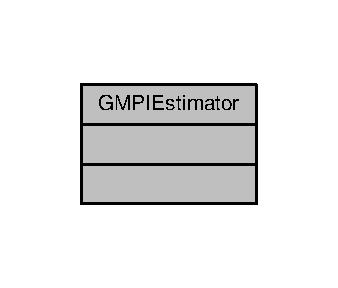
\includegraphics[width=162pt]{classGMPIEstimator__coll__graph}
\end{center}
\end{figure}


The documentation for this class was generated from the following file\-:\begin{DoxyCompactItemize}
\item 
\hyperlink{GMPIEstimator_8h}{G\-M\-P\-I\-Estimator.\-h}\end{DoxyCompactItemize}

\hypertarget{classVTKModelConstructor}{\section{V\-T\-K\-Model\-Constructor Class Reference}
\label{classVTKModelConstructor}\index{V\-T\-K\-Model\-Constructor@{V\-T\-K\-Model\-Constructor}}
}


{\ttfamily \#include $<$V\-T\-K\-Model\-Constructor.\-h$>$}



Collaboration diagram for V\-T\-K\-Model\-Constructor\-:
\nopagebreak
\begin{figure}[H]
\begin{center}
\leavevmode
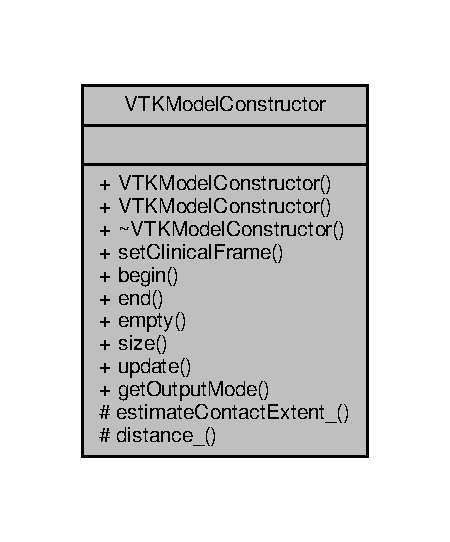
\includegraphics[width=216pt]{classVTKModelConstructor__coll__graph}
\end{center}
\end{figure}
\subsection*{Public Types}
\begin{DoxyCompactItemize}
\item 
typedef vector\\*
$<$ vtk\-Smart\-Pointer$<$ vtk\-Poly\-Data $>$\\*
 $>$\-::const\-\_\-iterator \hyperlink{classVTKModelConstructor_a439d0cca160eb72fc54c6727c69cbb5a}{Const\-Model\-Iterator}
\item 
typedef vector\\*
$<$ vtk\-Smart\-Pointer$<$ vtk\-Poly\-Data $>$\\*
 $>$\-::iterator \hyperlink{classVTKModelConstructor_a8ab5ac1866904faee9e4120b07f63701}{Model\-Iterator}
\end{DoxyCompactItemize}
\subsection*{Public Member Functions}
\begin{DoxyCompactItemize}
\item 
\hyperlink{classVTKModelConstructor_ad454bb3edb39bb81f7e8ea9580d31f05}{V\-T\-K\-Model\-Constructor} (const \hyperlink{classClinicalFrame}{Clinical\-Frame} $\ast$cf, bool s)
\item 
\hyperlink{classVTKModelConstructor_a6e08f2bba1f5b26d64f74ae64101e211}{V\-T\-K\-Model\-Constructor} (const \hyperlink{classClinicalFrame}{Clinical\-Frame} $\ast$cf)
\item 
\hyperlink{classVTKModelConstructor_accd2e4a9fce297452524424c56645af0}{$\sim$\-V\-T\-K\-Model\-Constructor} (void)
\item 
void \hyperlink{classVTKModelConstructor_a9661f98d603ca128f5bdf22ef78b15f1}{set\-Clinical\-Frame} (\hyperlink{classClinicalFrame}{Clinical\-Frame} $\ast$cf)
\item 
\hyperlink{classVTKModelConstructor_a8ab5ac1866904faee9e4120b07f63701}{Model\-Iterator} \hyperlink{classVTKModelConstructor_abd4236c1af1eb4c52dca9c89aa504555}{begin} (void)
\item 
\hyperlink{classVTKModelConstructor_a8ab5ac1866904faee9e4120b07f63701}{Model\-Iterator} \hyperlink{classVTKModelConstructor_a056e86cab4140ff9975d636de3a33486}{end} (void)
\item 
bool \hyperlink{classVTKModelConstructor_ac6f76a490e608339b6aa148089f535f7}{empty} (void)
\item 
int \hyperlink{classVTKModelConstructor_a5f939d68c9f15d8ec22ddb6a0c0090c7}{size} (void) const 
\item 
int \hyperlink{classVTKModelConstructor_ad6f6baa567097da53cbcaa91cf375531}{update} ()
\item 
bool \hyperlink{classVTKModelConstructor_aaec58670f5bb650109de05d2bbc5f8f1}{get\-Output\-Mode} (void) const 
\end{DoxyCompactItemize}
\subsection*{Protected Member Functions}
\begin{DoxyCompactItemize}
\item 
void \hyperlink{classVTKModelConstructor_a97c3716459da1a19e15a1b91283ccc8e}{estimate\-Contact\-Extent\-\_\-} (double $\ast$, double $\ast$, vtk\-Line\-Source $\ast$)
\item 
double \hyperlink{classVTKModelConstructor_a458e23ce8a24102118938f2ca18c8c2c}{distance\-\_\-} (double $\ast$p1, double $\ast$p2)
\end{DoxyCompactItemize}


\subsection{Detailed Description}
\hyperlink{classVTKModelConstructor}{V\-T\-K\-Model\-Constructor} class

This class constructs V\-T\-K 3\-D model based on reconstructed information 

\subsection{Member Typedef Documentation}
\hypertarget{classVTKModelConstructor_a439d0cca160eb72fc54c6727c69cbb5a}{\index{V\-T\-K\-Model\-Constructor@{V\-T\-K\-Model\-Constructor}!Const\-Model\-Iterator@{Const\-Model\-Iterator}}
\index{Const\-Model\-Iterator@{Const\-Model\-Iterator}!VTKModelConstructor@{V\-T\-K\-Model\-Constructor}}
\subsubsection[{Const\-Model\-Iterator}]{\setlength{\rightskip}{0pt plus 5cm}typedef vector$<$ vtk\-Smart\-Pointer$<$vtk\-Poly\-Data$>$ $>$\-::const\-\_\-iterator {\bf V\-T\-K\-Model\-Constructor\-::\-Const\-Model\-Iterator}}}\label{classVTKModelConstructor_a439d0cca160eb72fc54c6727c69cbb5a}
\hypertarget{classVTKModelConstructor_a8ab5ac1866904faee9e4120b07f63701}{\index{V\-T\-K\-Model\-Constructor@{V\-T\-K\-Model\-Constructor}!Model\-Iterator@{Model\-Iterator}}
\index{Model\-Iterator@{Model\-Iterator}!VTKModelConstructor@{V\-T\-K\-Model\-Constructor}}
\subsubsection[{Model\-Iterator}]{\setlength{\rightskip}{0pt plus 5cm}typedef vector$<$ vtk\-Smart\-Pointer$<$vtk\-Poly\-Data$>$ $>$\-::iterator {\bf V\-T\-K\-Model\-Constructor\-::\-Model\-Iterator}}}\label{classVTKModelConstructor_a8ab5ac1866904faee9e4120b07f63701}


\subsection{Constructor \& Destructor Documentation}
\hypertarget{classVTKModelConstructor_ad454bb3edb39bb81f7e8ea9580d31f05}{\index{V\-T\-K\-Model\-Constructor@{V\-T\-K\-Model\-Constructor}!V\-T\-K\-Model\-Constructor@{V\-T\-K\-Model\-Constructor}}
\index{V\-T\-K\-Model\-Constructor@{V\-T\-K\-Model\-Constructor}!VTKModelConstructor@{V\-T\-K\-Model\-Constructor}}
\subsubsection[{V\-T\-K\-Model\-Constructor}]{\setlength{\rightskip}{0pt plus 5cm}V\-T\-K\-Model\-Constructor\-::\-V\-T\-K\-Model\-Constructor (
\begin{DoxyParamCaption}
\item[{const {\bf Clinical\-Frame} $\ast$}]{cf, }
\item[{bool}]{s}
\end{DoxyParamCaption}
)\hspace{0.3cm}{\ttfamily [inline]}}}\label{classVTKModelConstructor_ad454bb3edb39bb81f7e8ea9580d31f05}

\begin{DoxyParams}{Parameters}
{\em cf} & holds the pointer to \hyperlink{classClinicalFrame}{Clinical\-Frame} and to vector$<$ Electrode $>$ \\
\hline
{\em c} & is a pointer to T\-C\-L\-A\-P\-::\-Cmd\-Line class to set/get command line options \\
\hline
\end{DoxyParams}
\hypertarget{classVTKModelConstructor_a6e08f2bba1f5b26d64f74ae64101e211}{\index{V\-T\-K\-Model\-Constructor@{V\-T\-K\-Model\-Constructor}!V\-T\-K\-Model\-Constructor@{V\-T\-K\-Model\-Constructor}}
\index{V\-T\-K\-Model\-Constructor@{V\-T\-K\-Model\-Constructor}!VTKModelConstructor@{V\-T\-K\-Model\-Constructor}}
\subsubsection[{V\-T\-K\-Model\-Constructor}]{\setlength{\rightskip}{0pt plus 5cm}V\-T\-K\-Model\-Constructor\-::\-V\-T\-K\-Model\-Constructor (
\begin{DoxyParamCaption}
\item[{const {\bf Clinical\-Frame} $\ast$}]{cf}
\end{DoxyParamCaption}
)\hspace{0.3cm}{\ttfamily [inline]}}}\label{classVTKModelConstructor_a6e08f2bba1f5b26d64f74ae64101e211}
\hypertarget{classVTKModelConstructor_accd2e4a9fce297452524424c56645af0}{\index{V\-T\-K\-Model\-Constructor@{V\-T\-K\-Model\-Constructor}!$\sim$\-V\-T\-K\-Model\-Constructor@{$\sim$\-V\-T\-K\-Model\-Constructor}}
\index{$\sim$\-V\-T\-K\-Model\-Constructor@{$\sim$\-V\-T\-K\-Model\-Constructor}!VTKModelConstructor@{V\-T\-K\-Model\-Constructor}}
\subsubsection[{$\sim$\-V\-T\-K\-Model\-Constructor}]{\setlength{\rightskip}{0pt plus 5cm}V\-T\-K\-Model\-Constructor\-::$\sim$\-V\-T\-K\-Model\-Constructor (
\begin{DoxyParamCaption}
\item[{void}]{}
\end{DoxyParamCaption}
)\hspace{0.3cm}{\ttfamily [inline]}}}\label{classVTKModelConstructor_accd2e4a9fce297452524424c56645af0}


\subsection{Member Function Documentation}
\hypertarget{classVTKModelConstructor_abd4236c1af1eb4c52dca9c89aa504555}{\index{V\-T\-K\-Model\-Constructor@{V\-T\-K\-Model\-Constructor}!begin@{begin}}
\index{begin@{begin}!VTKModelConstructor@{V\-T\-K\-Model\-Constructor}}
\subsubsection[{begin}]{\setlength{\rightskip}{0pt plus 5cm}{\bf Model\-Iterator} V\-T\-K\-Model\-Constructor\-::begin (
\begin{DoxyParamCaption}
\item[{void}]{}
\end{DoxyParamCaption}
)\hspace{0.3cm}{\ttfamily [inline]}}}\label{classVTKModelConstructor_abd4236c1af1eb4c52dca9c89aa504555}
methods that returns a pointer to the H\-E\-A\-D of V\-T\-K model vector \hypertarget{classVTKModelConstructor_a458e23ce8a24102118938f2ca18c8c2c}{\index{V\-T\-K\-Model\-Constructor@{V\-T\-K\-Model\-Constructor}!distance\-\_\-@{distance\-\_\-}}
\index{distance\-\_\-@{distance\-\_\-}!VTKModelConstructor@{V\-T\-K\-Model\-Constructor}}
\subsubsection[{distance\-\_\-}]{\setlength{\rightskip}{0pt plus 5cm}double V\-T\-K\-Model\-Constructor\-::distance\-\_\- (
\begin{DoxyParamCaption}
\item[{double $\ast$}]{p1, }
\item[{double $\ast$}]{p2}
\end{DoxyParamCaption}
)\hspace{0.3cm}{\ttfamily [protected]}}}\label{classVTKModelConstructor_a458e23ce8a24102118938f2ca18c8c2c}
function that computes the euclidean distance between two points \hypertarget{classVTKModelConstructor_ac6f76a490e608339b6aa148089f535f7}{\index{V\-T\-K\-Model\-Constructor@{V\-T\-K\-Model\-Constructor}!empty@{empty}}
\index{empty@{empty}!VTKModelConstructor@{V\-T\-K\-Model\-Constructor}}
\subsubsection[{empty}]{\setlength{\rightskip}{0pt plus 5cm}bool V\-T\-K\-Model\-Constructor\-::empty (
\begin{DoxyParamCaption}
\item[{void}]{}
\end{DoxyParamCaption}
)\hspace{0.3cm}{\ttfamily [inline]}}}\label{classVTKModelConstructor_ac6f76a490e608339b6aa148089f535f7}
methods that check whether V\-T\-K model vector is empty \hypertarget{classVTKModelConstructor_a056e86cab4140ff9975d636de3a33486}{\index{V\-T\-K\-Model\-Constructor@{V\-T\-K\-Model\-Constructor}!end@{end}}
\index{end@{end}!VTKModelConstructor@{V\-T\-K\-Model\-Constructor}}
\subsubsection[{end}]{\setlength{\rightskip}{0pt plus 5cm}{\bf Model\-Iterator} V\-T\-K\-Model\-Constructor\-::end (
\begin{DoxyParamCaption}
\item[{void}]{}
\end{DoxyParamCaption}
)\hspace{0.3cm}{\ttfamily [inline]}}}\label{classVTKModelConstructor_a056e86cab4140ff9975d636de3a33486}
methods that returns a pointer to the T\-A\-I\-L of V\-T\-K model vector \hypertarget{classVTKModelConstructor_a97c3716459da1a19e15a1b91283ccc8e}{\index{V\-T\-K\-Model\-Constructor@{V\-T\-K\-Model\-Constructor}!estimate\-Contact\-Extent\-\_\-@{estimate\-Contact\-Extent\-\_\-}}
\index{estimate\-Contact\-Extent\-\_\-@{estimate\-Contact\-Extent\-\_\-}!VTKModelConstructor@{V\-T\-K\-Model\-Constructor}}
\subsubsection[{estimate\-Contact\-Extent\-\_\-}]{\setlength{\rightskip}{0pt plus 5cm}void V\-T\-K\-Model\-Constructor\-::estimate\-Contact\-Extent\-\_\- (
\begin{DoxyParamCaption}
\item[{double $\ast$}]{p1, }
\item[{double $\ast$}]{p2, }
\item[{vtk\-Line\-Source $\ast$}]{line}
\end{DoxyParamCaption}
)\hspace{0.3cm}{\ttfamily [protected]}}}\label{classVTKModelConstructor_a97c3716459da1a19e15a1b91283ccc8e}
for each contact it estimates its position along the line that connectes contact1 and contact2 A\-T\-M the function assumes that p1 and p2 are 3.\-5 mm apart, better estimation needs to be used in order to create more physically reliable models \hypertarget{classVTKModelConstructor_aaec58670f5bb650109de05d2bbc5f8f1}{\index{V\-T\-K\-Model\-Constructor@{V\-T\-K\-Model\-Constructor}!get\-Output\-Mode@{get\-Output\-Mode}}
\index{get\-Output\-Mode@{get\-Output\-Mode}!VTKModelConstructor@{V\-T\-K\-Model\-Constructor}}
\subsubsection[{get\-Output\-Mode}]{\setlength{\rightskip}{0pt plus 5cm}bool V\-T\-K\-Model\-Constructor\-::get\-Output\-Mode (
\begin{DoxyParamCaption}
\item[{void}]{}
\end{DoxyParamCaption}
) const\hspace{0.3cm}{\ttfamily [inline]}}}\label{classVTKModelConstructor_aaec58670f5bb650109de05d2bbc5f8f1}
this function returns whether the user requested a single vtk file (ie all the electrodes together as output or multiple files (ie each electrode as separate vtk file) \hypertarget{classVTKModelConstructor_a9661f98d603ca128f5bdf22ef78b15f1}{\index{V\-T\-K\-Model\-Constructor@{V\-T\-K\-Model\-Constructor}!set\-Clinical\-Frame@{set\-Clinical\-Frame}}
\index{set\-Clinical\-Frame@{set\-Clinical\-Frame}!VTKModelConstructor@{V\-T\-K\-Model\-Constructor}}
\subsubsection[{set\-Clinical\-Frame}]{\setlength{\rightskip}{0pt plus 5cm}void V\-T\-K\-Model\-Constructor\-::set\-Clinical\-Frame (
\begin{DoxyParamCaption}
\item[{{\bf Clinical\-Frame} $\ast$}]{cf}
\end{DoxyParamCaption}
)\hspace{0.3cm}{\ttfamily [inline]}}}\label{classVTKModelConstructor_a9661f98d603ca128f5bdf22ef78b15f1}
\hypertarget{classVTKModelConstructor_a5f939d68c9f15d8ec22ddb6a0c0090c7}{\index{V\-T\-K\-Model\-Constructor@{V\-T\-K\-Model\-Constructor}!size@{size}}
\index{size@{size}!VTKModelConstructor@{V\-T\-K\-Model\-Constructor}}
\subsubsection[{size}]{\setlength{\rightskip}{0pt plus 5cm}int V\-T\-K\-Model\-Constructor\-::size (
\begin{DoxyParamCaption}
\item[{void}]{}
\end{DoxyParamCaption}
) const\hspace{0.3cm}{\ttfamily [inline]}}}\label{classVTKModelConstructor_a5f939d68c9f15d8ec22ddb6a0c0090c7}
\hypertarget{classVTKModelConstructor_ad6f6baa567097da53cbcaa91cf375531}{\index{V\-T\-K\-Model\-Constructor@{V\-T\-K\-Model\-Constructor}!update@{update}}
\index{update@{update}!VTKModelConstructor@{V\-T\-K\-Model\-Constructor}}
\subsubsection[{update}]{\setlength{\rightskip}{0pt plus 5cm}int V\-T\-K\-Model\-Constructor\-::update (
\begin{DoxyParamCaption}
\item[{void}]{}
\end{DoxyParamCaption}
)}}\label{classVTKModelConstructor_ad6f6baa567097da53cbcaa91cf375531}
function that computes the euclidean distance between two points core method that navigate the clinical frame, extracts the centroids for each contact, estimates the contact as well as the electrode axes, and builds the vtk model (cylinder + spline) based on reconstructed information \begin{DoxyReturn}{Returns}
this function returns 0 or 1 upon failure or success, respectively 
\end{DoxyReturn}


The documentation for this class was generated from the following file\-:\begin{DoxyCompactItemize}
\item 
\hyperlink{VTKModelConstructor_8h}{V\-T\-K\-Model\-Constructor.\-h}\end{DoxyCompactItemize}

\hypertarget{classVTKWriter}{\section{V\-T\-K\-Writer Class Reference}
\label{classVTKWriter}\index{V\-T\-K\-Writer@{V\-T\-K\-Writer}}
}


{\ttfamily \#include $<$V\-T\-K\-Writer.\-h$>$}



Inheritance diagram for V\-T\-K\-Writer\-:
\nopagebreak
\begin{figure}[H]
\begin{center}
\leavevmode
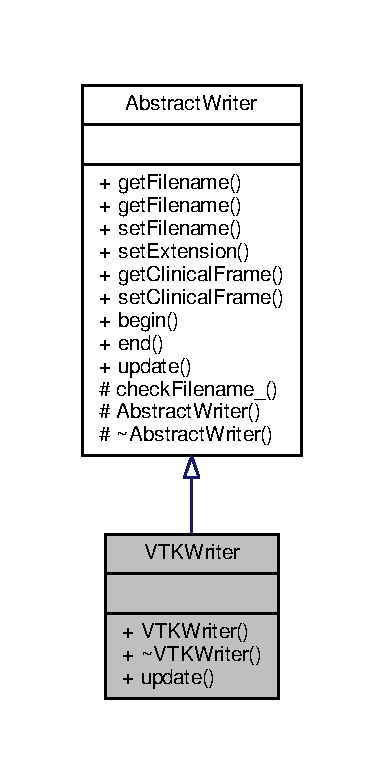
\includegraphics[width=184pt]{classVTKWriter__inherit__graph}
\end{center}
\end{figure}


Collaboration diagram for V\-T\-K\-Writer\-:
\nopagebreak
\begin{figure}[H]
\begin{center}
\leavevmode
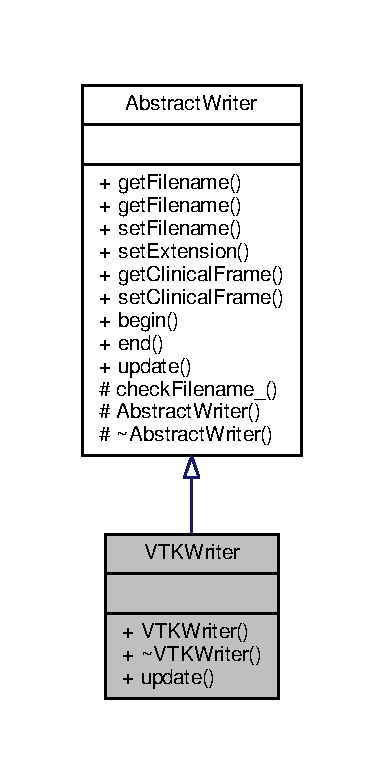
\includegraphics[width=184pt]{classVTKWriter__coll__graph}
\end{center}
\end{figure}
\subsection*{Public Member Functions}
\begin{DoxyCompactItemize}
\item 
\hyperlink{classVTKWriter_a5dc5c66ce133cee517c90552d5a5f9c4}{V\-T\-K\-Writer} (string filename, T\-C\-L\-A\-P\-::\-Cmd\-Line \&c)
\item 
virtual \hyperlink{classVTKWriter_afe21ea45991aadd03d20dbd94e167839}{$\sim$\-V\-T\-K\-Writer} (void)
\item 
int \hyperlink{classVTKWriter_abb335d732c6dceac1a389e118e7afb6c}{update} ()
\end{DoxyCompactItemize}
\subsection*{Additional Inherited Members}


\subsection{Detailed Description}
\hyperlink{classVTKWriter}{V\-T\-K\-Writer} class 

\subsection{Constructor \& Destructor Documentation}
\hypertarget{classVTKWriter_a5dc5c66ce133cee517c90552d5a5f9c4}{\index{V\-T\-K\-Writer@{V\-T\-K\-Writer}!V\-T\-K\-Writer@{V\-T\-K\-Writer}}
\index{V\-T\-K\-Writer@{V\-T\-K\-Writer}!VTKWriter@{V\-T\-K\-Writer}}
\subsubsection[{V\-T\-K\-Writer}]{\setlength{\rightskip}{0pt plus 5cm}V\-T\-K\-Writer\-::\-V\-T\-K\-Writer (
\begin{DoxyParamCaption}
\item[{string}]{filename, }
\item[{T\-C\-L\-A\-P\-::\-Cmd\-Line \&}]{c}
\end{DoxyParamCaption}
)\hspace{0.3cm}{\ttfamily [inline]}}}\label{classVTKWriter_a5dc5c66ce133cee517c90552d5a5f9c4}
\hypertarget{classVTKWriter_afe21ea45991aadd03d20dbd94e167839}{\index{V\-T\-K\-Writer@{V\-T\-K\-Writer}!$\sim$\-V\-T\-K\-Writer@{$\sim$\-V\-T\-K\-Writer}}
\index{$\sim$\-V\-T\-K\-Writer@{$\sim$\-V\-T\-K\-Writer}!VTKWriter@{V\-T\-K\-Writer}}
\subsubsection[{$\sim$\-V\-T\-K\-Writer}]{\setlength{\rightskip}{0pt plus 5cm}virtual V\-T\-K\-Writer\-::$\sim$\-V\-T\-K\-Writer (
\begin{DoxyParamCaption}
\item[{void}]{}
\end{DoxyParamCaption}
)\hspace{0.3cm}{\ttfamily [inline]}, {\ttfamily [virtual]}}}\label{classVTKWriter_afe21ea45991aadd03d20dbd94e167839}


\subsection{Member Function Documentation}
\hypertarget{classVTKWriter_abb335d732c6dceac1a389e118e7afb6c}{\index{V\-T\-K\-Writer@{V\-T\-K\-Writer}!update@{update}}
\index{update@{update}!VTKWriter@{V\-T\-K\-Writer}}
\subsubsection[{update}]{\setlength{\rightskip}{0pt plus 5cm}int V\-T\-K\-Writer\-::update (
\begin{DoxyParamCaption}
\item[{void}]{}
\end{DoxyParamCaption}
)\hspace{0.3cm}{\ttfamily [virtual]}}}\label{classVTKWriter_abb335d732c6dceac1a389e118e7afb6c}
implementation of virtual Abstract\-File\-Writer\-::update This function navigate through vtk\-Model\-Constructor output and writes them down 

Implements \hyperlink{classAbstractWriter_ae3d1e946840352b28b092902664a1115}{Abstract\-Writer}.



The documentation for this class was generated from the following file\-:\begin{DoxyCompactItemize}
\item 
\hyperlink{VTKWriter_8h}{V\-T\-K\-Writer.\-h}\end{DoxyCompactItemize}

\chapter{File Documentation}
\hypertarget{AbstractWriter_8h}{\section{Abstract\-Writer.\-h File Reference}
\label{AbstractWriter_8h}\index{Abstract\-Writer.\-h@{Abstract\-Writer.\-h}}
}
{\ttfamily \#include \char`\"{}Definitions.\-h\char`\"{}}\\*
{\ttfamily \#include \char`\"{}Clinical\-Frame.\-h\char`\"{}}\\*
Include dependency graph for Abstract\-Writer.\-h\-:
\nopagebreak
\begin{figure}[H]
\begin{center}
\leavevmode
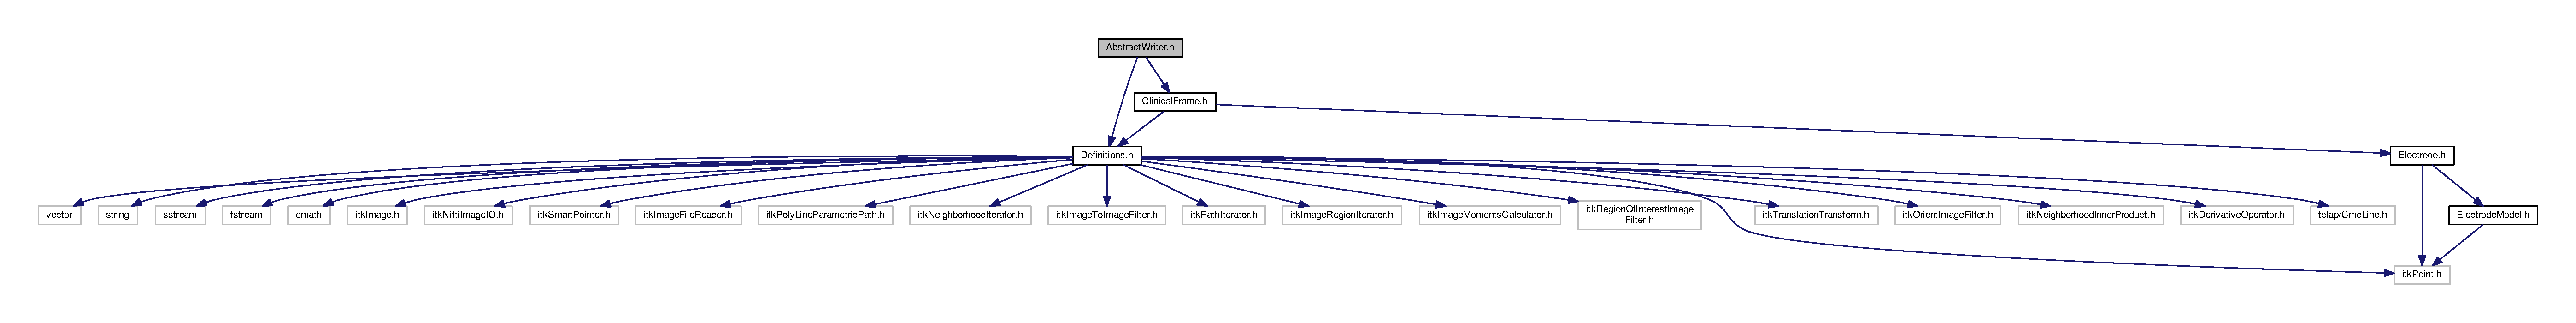
\includegraphics[width=350pt]{AbstractWriter_8h__incl}
\end{center}
\end{figure}
This graph shows which files directly or indirectly include this file\-:
\nopagebreak
\begin{figure}[H]
\begin{center}
\leavevmode
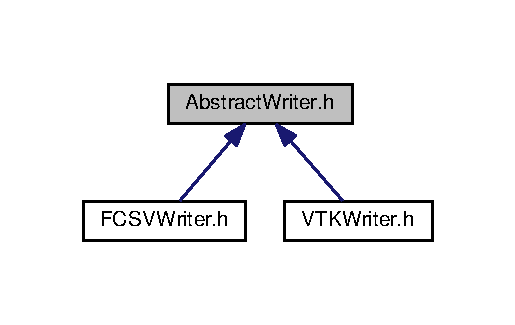
\includegraphics[width=247pt]{AbstractWriter_8h__dep__incl}
\end{center}
\end{figure}
\subsection*{Classes}
\begin{DoxyCompactItemize}
\item 
class \hyperlink{classAbstractWriter}{Abstract\-Writer}
\end{DoxyCompactItemize}

\hypertarget{AnatomicalPatchBuilder_8h}{\section{Anatomical\-Patch\-Builder.\-h File Reference}
\label{AnatomicalPatchBuilder_8h}\index{Anatomical\-Patch\-Builder.\-h@{Anatomical\-Patch\-Builder.\-h}}
}
\subsection*{Classes}
\begin{DoxyCompactItemize}
\item 
class \hyperlink{classAnatomicalPatchBuilder_3_01class_01T_01_4}{Anatomical\-Patch\-Builder$<$ class T $>$}
\end{DoxyCompactItemize}

\hypertarget{ClinicalFrame_8h}{\section{Clinical\-Frame.\-h File Reference}
\label{ClinicalFrame_8h}\index{Clinical\-Frame.\-h@{Clinical\-Frame.\-h}}
}
{\ttfamily \#include $<$Definitions.\-h$>$}\\*
{\ttfamily \#include $<$Electrode.\-h$>$}\\*
Include dependency graph for Clinical\-Frame.\-h\-:
\nopagebreak
\begin{figure}[H]
\begin{center}
\leavevmode
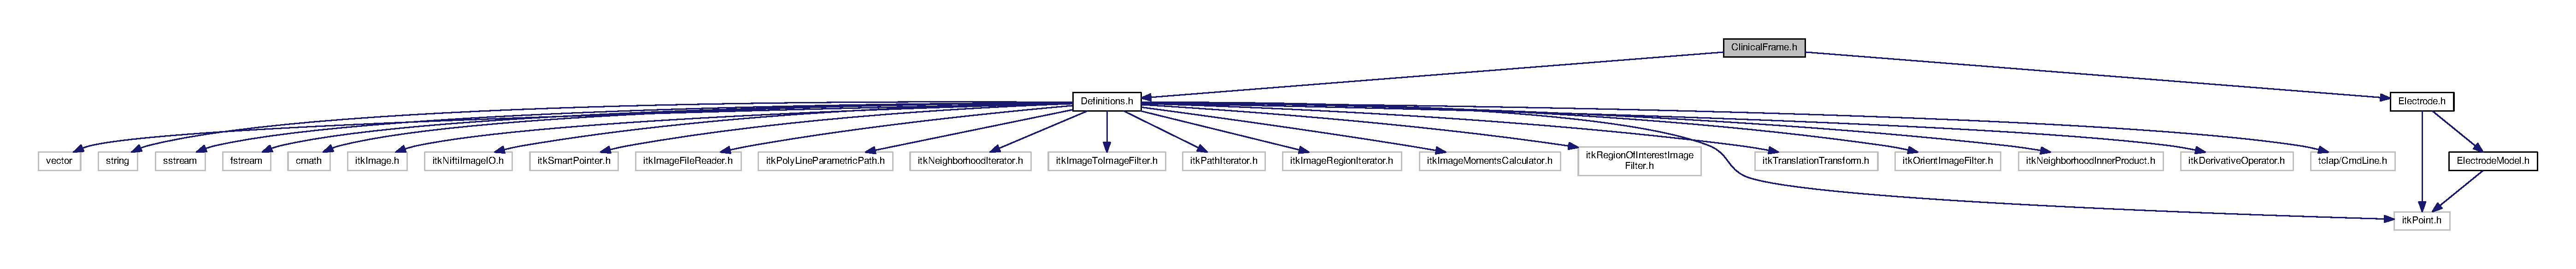
\includegraphics[width=350pt]{ClinicalFrame_8h__incl}
\end{center}
\end{figure}
This graph shows which files directly or indirectly include this file\-:
\nopagebreak
\begin{figure}[H]
\begin{center}
\leavevmode
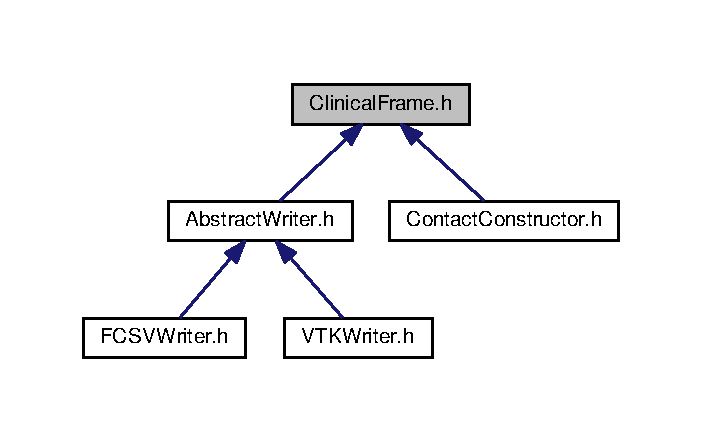
\includegraphics[width=337pt]{ClinicalFrame_8h__dep__incl}
\end{center}
\end{figure}
\subsection*{Classes}
\begin{DoxyCompactItemize}
\item 
class \hyperlink{classClinicalFrame}{Clinical\-Frame}
\end{DoxyCompactItemize}

\hypertarget{ContactConstructor_8h}{\section{Contact\-Constructor.\-h File Reference}
\label{ContactConstructor_8h}\index{Contact\-Constructor.\-h@{Contact\-Constructor.\-h}}
}
{\ttfamily \#include \char`\"{}Definitions.\-h\char`\"{}}\\*
{\ttfamily \#include \char`\"{}Electrode.\-h\char`\"{}}\\*
{\ttfamily \#include \char`\"{}Clinical\-Frame.\-h\char`\"{}}\\*
{\ttfamily \#include \char`\"{}itk\-Image\-To\-List\-Sample\-Adaptor.\-h\char`\"{}}\\*
{\ttfamily \#include \char`\"{}itk\-Histogram.\-h\char`\"{}}\\*
{\ttfamily \#include \char`\"{}itk\-Sample\-To\-Histogram\-Filter.\-h\char`\"{}}\\*
{\ttfamily \#include \char`\"{}itk\-Minimum\-Maximum\-Image\-Calculator.\-h\char`\"{}}\\*
Include dependency graph for Contact\-Constructor.\-h\-:
\nopagebreak
\begin{figure}[H]
\begin{center}
\leavevmode
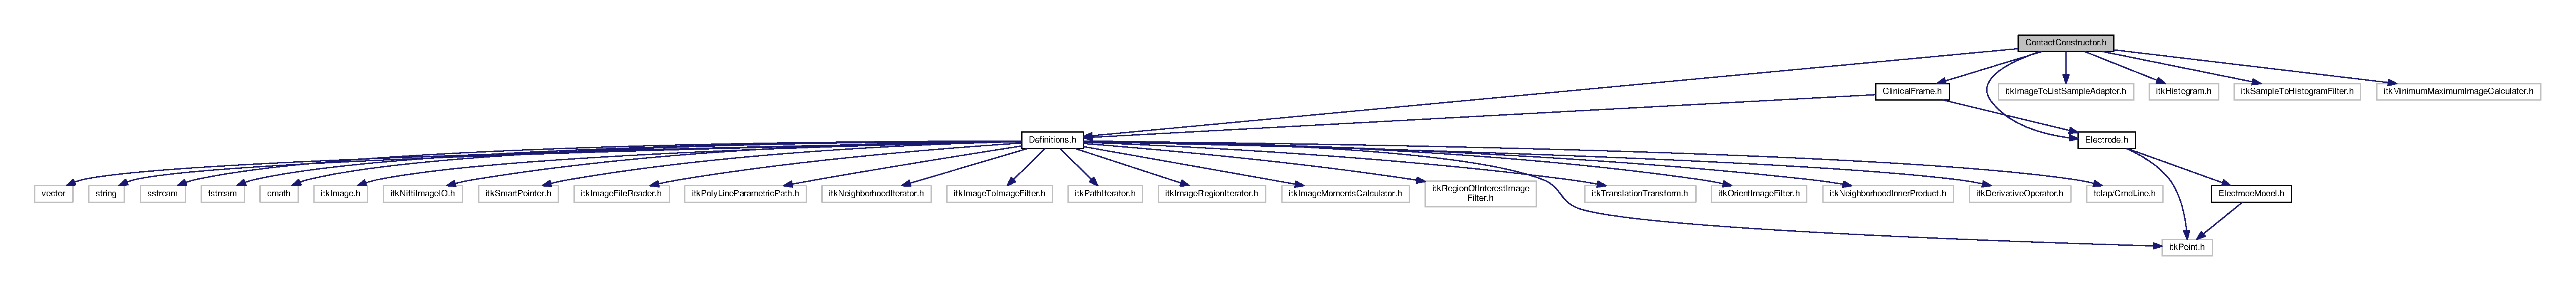
\includegraphics[width=350pt]{ContactConstructor_8h__incl}
\end{center}
\end{figure}
\subsection*{Classes}
\begin{DoxyCompactItemize}
\item 
class \hyperlink{classContactConstructor}{Contact\-Constructor}
\end{DoxyCompactItemize}

\hypertarget{Definitions_8h}{\section{Definitions.\-h File Reference}
\label{Definitions_8h}\index{Definitions.\-h@{Definitions.\-h}}
}
{\ttfamily \#include $<$vector$>$}\\*
{\ttfamily \#include $<$string$>$}\\*
{\ttfamily \#include $<$sstream$>$}\\*
{\ttfamily \#include $<$fstream$>$}\\*
{\ttfamily \#include $<$cmath$>$}\\*
{\ttfamily \#include $<$itk\-Image.\-h$>$}\\*
{\ttfamily \#include $<$itk\-Nifti\-Image\-I\-O.\-h$>$}\\*
{\ttfamily \#include $<$itk\-Smart\-Pointer.\-h$>$}\\*
{\ttfamily \#include $<$itk\-Image\-File\-Reader.\-h$>$}\\*
{\ttfamily \#include $<$itk\-Poly\-Line\-Parametric\-Path.\-h$>$}\\*
{\ttfamily \#include $<$itk\-Neighborhood\-Iterator.\-h$>$}\\*
{\ttfamily \#include $<$itk\-Image\-To\-Image\-Filter.\-h$>$}\\*
{\ttfamily \#include $<$itk\-Path\-Iterator.\-h$>$}\\*
{\ttfamily \#include $<$itk\-Image\-Region\-Iterator.\-h$>$}\\*
{\ttfamily \#include $<$itk\-Image\-Moments\-Calculator.\-h$>$}\\*
{\ttfamily \#include $<$itk\-Region\-Of\-Interest\-Image\-Filter.\-h$>$}\\*
{\ttfamily \#include $<$itk\-Point.\-h$>$}\\*
{\ttfamily \#include $<$itk\-Translation\-Transform.\-h$>$}\\*
{\ttfamily \#include $<$itk\-Orient\-Image\-Filter.\-h$>$}\\*
{\ttfamily \#include $<$itk\-Neighborhood\-Inner\-Product.\-h$>$}\\*
{\ttfamily \#include $<$itk\-Derivative\-Operator.\-h$>$}\\*
{\ttfamily \#include $<$tclap/\-Cmd\-Line.\-h$>$}\\*
Include dependency graph for Definitions.\-h\-:
\nopagebreak
\begin{figure}[H]
\begin{center}
\leavevmode
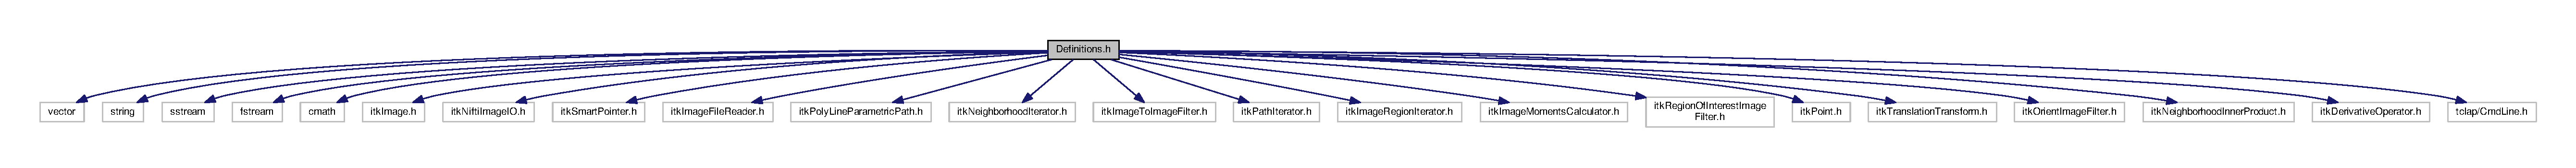
\includegraphics[width=350pt]{Definitions_8h__incl}
\end{center}
\end{figure}
This graph shows which files directly or indirectly include this file\-:
\nopagebreak
\begin{figure}[H]
\begin{center}
\leavevmode
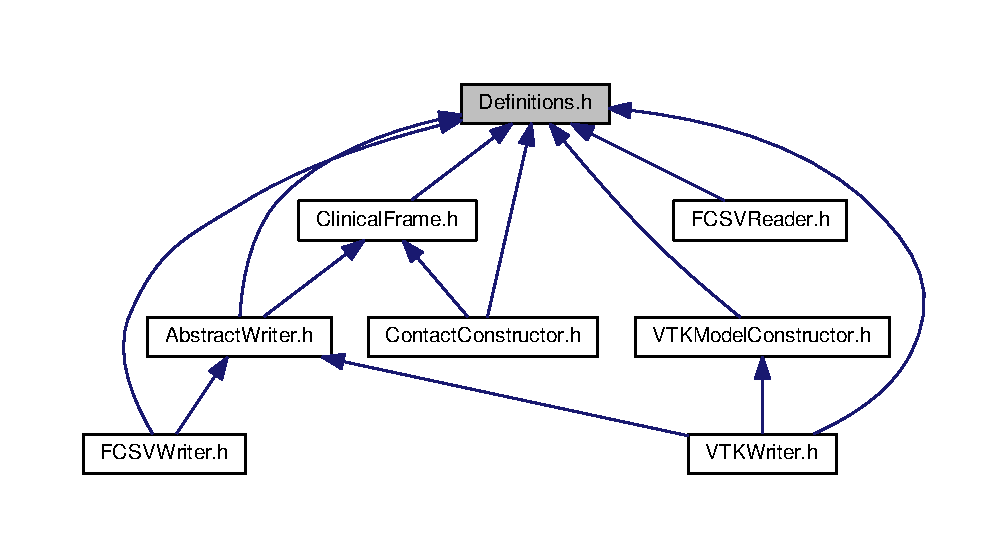
\includegraphics[width=350pt]{Definitions_8h__dep__incl}
\end{center}
\end{figure}
\subsection*{Typedefs}
\begin{DoxyCompactItemize}
\item 
typedef itk\-::\-Image$<$ short, 3 $>$ \hyperlink{Definitions_8h_a802532dc139f219ffb61a72f80eb304a}{Image\-Type}
\item 
typedef Image\-Type\-::\-Pointer \hyperlink{Definitions_8h_a6952b2a622249cc460a5875f2a793e61}{Image\-Pointer\-Type}
\item 
typedef itk\-::\-Point$<$ double, 3 $>$ \hyperlink{Definitions_8h_ab9d62e9721984f22424e47212a5ce25d}{Physical\-Point\-Type}
\item 
typedef Image\-Type\-::\-Index\-Type \hyperlink{Definitions_8h_ae685a5b33fd611f035ca2e96f295ff01}{Voxel\-Point\-Type}
\item 
typedef itk\-::\-Image\-File\-Reader\\*
$<$ \hyperlink{Definitions_8h_a802532dc139f219ffb61a72f80eb304a}{Image\-Type} $>$ \hyperlink{Definitions_8h_a9e26f526b940bed527c826dc95a3bb50}{Image\-Reader\-Type}
\item 
typedef \\*
itk\-::\-Image\-Moments\-Calculator\\*
$<$ \hyperlink{Definitions_8h_a802532dc139f219ffb61a72f80eb304a}{Image\-Type} $>$ \hyperlink{Definitions_8h_ac94116121a5106707a88c6e919d080f8}{Calculator\-Type}
\item 
typedef Image\-Type\-::\-Size\-Type \hyperlink{Definitions_8h_a54604dadf3bd1e5feb73fc752d64a349}{Size\-Type}
\item 
typedef Image\-Type\-::\-Region\-Type \hyperlink{Definitions_8h_aa43cbdad7eb11c22fc56724b2662ff77}{Region\-Type}
\item 
typedef Image\-Type\-::\-Spacing\-Type \hyperlink{Definitions_8h_acdd20dc566401809116845da40ffdc4e}{Spacing\-Type}
\item 
typedef \\*
itk\-::\-Region\-Of\-Interest\-Image\-Filter\\*
$<$ \hyperlink{Definitions_8h_a802532dc139f219ffb61a72f80eb304a}{Image\-Type}, \hyperlink{Definitions_8h_a802532dc139f219ffb61a72f80eb304a}{Image\-Type} $>$ \hyperlink{Definitions_8h_a678719635ee6db0a8cd68bd56bcdec02}{Filter\-Type}
\end{DoxyCompactItemize}


\subsection{Typedef Documentation}
\hypertarget{Definitions_8h_ac94116121a5106707a88c6e919d080f8}{\index{Definitions.\-h@{Definitions.\-h}!Calculator\-Type@{Calculator\-Type}}
\index{Calculator\-Type@{Calculator\-Type}!Definitions.h@{Definitions.\-h}}
\subsubsection[{Calculator\-Type}]{\setlength{\rightskip}{0pt plus 5cm}typedef itk\-::\-Image\-Moments\-Calculator$<${\bf Image\-Type}$>$ {\bf Calculator\-Type}}}\label{Definitions_8h_ac94116121a5106707a88c6e919d080f8}
\hypertarget{Definitions_8h_a678719635ee6db0a8cd68bd56bcdec02}{\index{Definitions.\-h@{Definitions.\-h}!Filter\-Type@{Filter\-Type}}
\index{Filter\-Type@{Filter\-Type}!Definitions.h@{Definitions.\-h}}
\subsubsection[{Filter\-Type}]{\setlength{\rightskip}{0pt plus 5cm}typedef itk\-::\-Region\-Of\-Interest\-Image\-Filter$<${\bf Image\-Type},{\bf Image\-Type}$>$ {\bf Filter\-Type}}}\label{Definitions_8h_a678719635ee6db0a8cd68bd56bcdec02}
\hypertarget{Definitions_8h_a6952b2a622249cc460a5875f2a793e61}{\index{Definitions.\-h@{Definitions.\-h}!Image\-Pointer\-Type@{Image\-Pointer\-Type}}
\index{Image\-Pointer\-Type@{Image\-Pointer\-Type}!Definitions.h@{Definitions.\-h}}
\subsubsection[{Image\-Pointer\-Type}]{\setlength{\rightskip}{0pt plus 5cm}typedef Image\-Type\-::\-Pointer {\bf Image\-Pointer\-Type}}}\label{Definitions_8h_a6952b2a622249cc460a5875f2a793e61}
\hypertarget{Definitions_8h_a9e26f526b940bed527c826dc95a3bb50}{\index{Definitions.\-h@{Definitions.\-h}!Image\-Reader\-Type@{Image\-Reader\-Type}}
\index{Image\-Reader\-Type@{Image\-Reader\-Type}!Definitions.h@{Definitions.\-h}}
\subsubsection[{Image\-Reader\-Type}]{\setlength{\rightskip}{0pt plus 5cm}typedef itk\-::\-Image\-File\-Reader$<$ {\bf Image\-Type} $>$ {\bf Image\-Reader\-Type}}}\label{Definitions_8h_a9e26f526b940bed527c826dc95a3bb50}
\hypertarget{Definitions_8h_a802532dc139f219ffb61a72f80eb304a}{\index{Definitions.\-h@{Definitions.\-h}!Image\-Type@{Image\-Type}}
\index{Image\-Type@{Image\-Type}!Definitions.h@{Definitions.\-h}}
\subsubsection[{Image\-Type}]{\setlength{\rightskip}{0pt plus 5cm}typedef itk\-::\-Image$<$short, 3$>$ {\bf Image\-Type}}}\label{Definitions_8h_a802532dc139f219ffb61a72f80eb304a}
\hypertarget{Definitions_8h_ab9d62e9721984f22424e47212a5ce25d}{\index{Definitions.\-h@{Definitions.\-h}!Physical\-Point\-Type@{Physical\-Point\-Type}}
\index{Physical\-Point\-Type@{Physical\-Point\-Type}!Definitions.h@{Definitions.\-h}}
\subsubsection[{Physical\-Point\-Type}]{\setlength{\rightskip}{0pt plus 5cm}typedef itk\-::\-Point$<$double,3$>$ {\bf Physical\-Point\-Type}}}\label{Definitions_8h_ab9d62e9721984f22424e47212a5ce25d}
\hypertarget{Definitions_8h_aa43cbdad7eb11c22fc56724b2662ff77}{\index{Definitions.\-h@{Definitions.\-h}!Region\-Type@{Region\-Type}}
\index{Region\-Type@{Region\-Type}!Definitions.h@{Definitions.\-h}}
\subsubsection[{Region\-Type}]{\setlength{\rightskip}{0pt plus 5cm}typedef Image\-Type\-::\-Region\-Type {\bf Region\-Type}}}\label{Definitions_8h_aa43cbdad7eb11c22fc56724b2662ff77}
\hypertarget{Definitions_8h_a54604dadf3bd1e5feb73fc752d64a349}{\index{Definitions.\-h@{Definitions.\-h}!Size\-Type@{Size\-Type}}
\index{Size\-Type@{Size\-Type}!Definitions.h@{Definitions.\-h}}
\subsubsection[{Size\-Type}]{\setlength{\rightskip}{0pt plus 5cm}typedef Image\-Type\-::\-Size\-Type {\bf Size\-Type}}}\label{Definitions_8h_a54604dadf3bd1e5feb73fc752d64a349}
\hypertarget{Definitions_8h_acdd20dc566401809116845da40ffdc4e}{\index{Definitions.\-h@{Definitions.\-h}!Spacing\-Type@{Spacing\-Type}}
\index{Spacing\-Type@{Spacing\-Type}!Definitions.h@{Definitions.\-h}}
\subsubsection[{Spacing\-Type}]{\setlength{\rightskip}{0pt plus 5cm}typedef Image\-Type\-::\-Spacing\-Type {\bf Spacing\-Type}}}\label{Definitions_8h_acdd20dc566401809116845da40ffdc4e}
\hypertarget{Definitions_8h_ae685a5b33fd611f035ca2e96f295ff01}{\index{Definitions.\-h@{Definitions.\-h}!Voxel\-Point\-Type@{Voxel\-Point\-Type}}
\index{Voxel\-Point\-Type@{Voxel\-Point\-Type}!Definitions.h@{Definitions.\-h}}
\subsubsection[{Voxel\-Point\-Type}]{\setlength{\rightskip}{0pt plus 5cm}typedef Image\-Type\-::\-Index\-Type {\bf Voxel\-Point\-Type}}}\label{Definitions_8h_ae685a5b33fd611f035ca2e96f295ff01}

\hypertarget{Electrode_8h}{\section{Electrode.\-h File Reference}
\label{Electrode_8h}\index{Electrode.\-h@{Electrode.\-h}}
}
{\ttfamily \#include $<$itk\-Point.\-h$>$}\\*
{\ttfamily \#include \char`\"{}Electrode\-Model.\-h\char`\"{}}\\*
Include dependency graph for Electrode.\-h\-:
\nopagebreak
\begin{figure}[H]
\begin{center}
\leavevmode
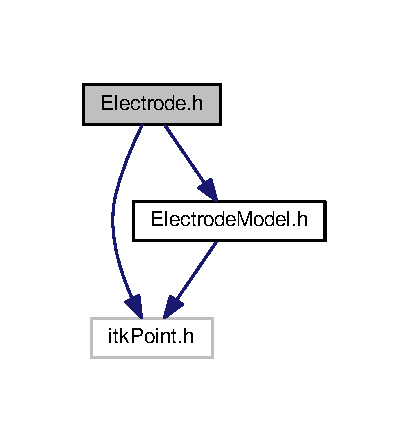
\includegraphics[width=196pt]{Electrode_8h__incl}
\end{center}
\end{figure}
This graph shows which files directly or indirectly include this file\-:
\nopagebreak
\begin{figure}[H]
\begin{center}
\leavevmode
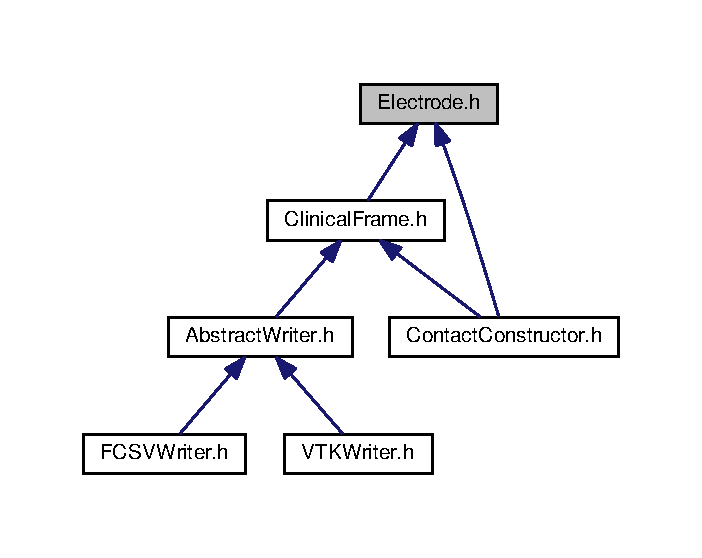
\includegraphics[width=337pt]{Electrode_8h__dep__incl}
\end{center}
\end{figure}
\subsection*{Classes}
\begin{DoxyCompactItemize}
\item 
class \hyperlink{classElectrode}{Electrode}
\end{DoxyCompactItemize}

\hypertarget{ElectrodeModel_8h}{\section{Electrode\-Model.\-h File Reference}
\label{ElectrodeModel_8h}\index{Electrode\-Model.\-h@{Electrode\-Model.\-h}}
}
{\ttfamily \#include $<$itk\-Point.\-h$>$}\\*
Include dependency graph for Electrode\-Model.\-h\-:
\nopagebreak
\begin{figure}[H]
\begin{center}
\leavevmode
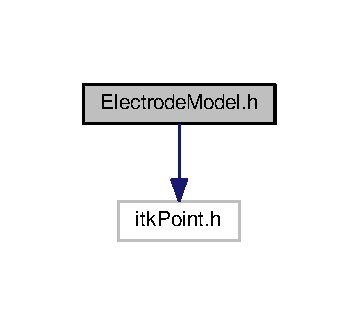
\includegraphics[width=172pt]{ElectrodeModel_8h__incl}
\end{center}
\end{figure}
This graph shows which files directly or indirectly include this file\-:
\nopagebreak
\begin{figure}[H]
\begin{center}
\leavevmode
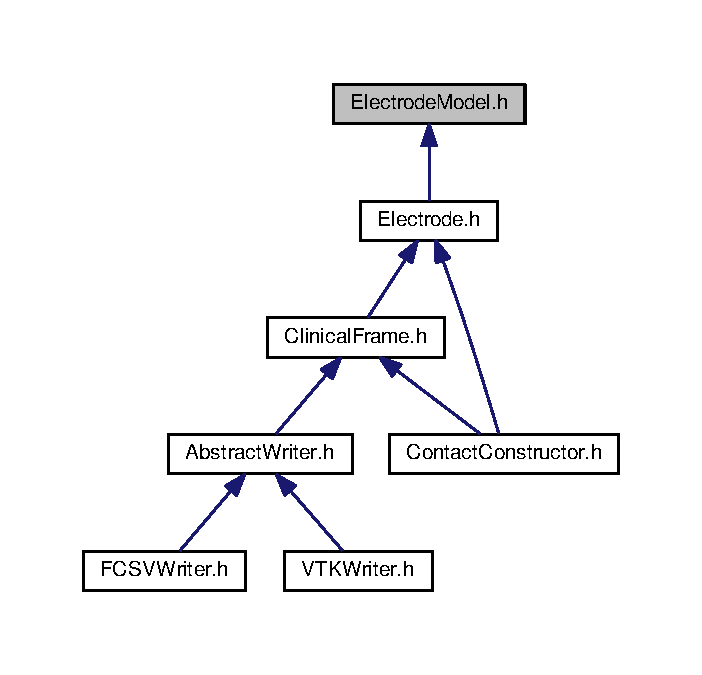
\includegraphics[width=337pt]{ElectrodeModel_8h__dep__incl}
\end{center}
\end{figure}
\subsection*{Classes}
\begin{DoxyCompactItemize}
\item 
class \hyperlink{classElectrodeModel}{Electrode\-Model}
\end{DoxyCompactItemize}

\hypertarget{FCSVReader_8h}{\section{F\-C\-S\-V\-Reader.\-h File Reference}
\label{FCSVReader_8h}\index{F\-C\-S\-V\-Reader.\-h@{F\-C\-S\-V\-Reader.\-h}}
}
{\ttfamily \#include $<$Definitions.\-h$>$}\\*
{\ttfamily \#include $<$tclap/\-Cmd\-Line.\-h$>$}\\*
Include dependency graph for F\-C\-S\-V\-Reader.\-h\-:
\nopagebreak
\begin{figure}[H]
\begin{center}
\leavevmode
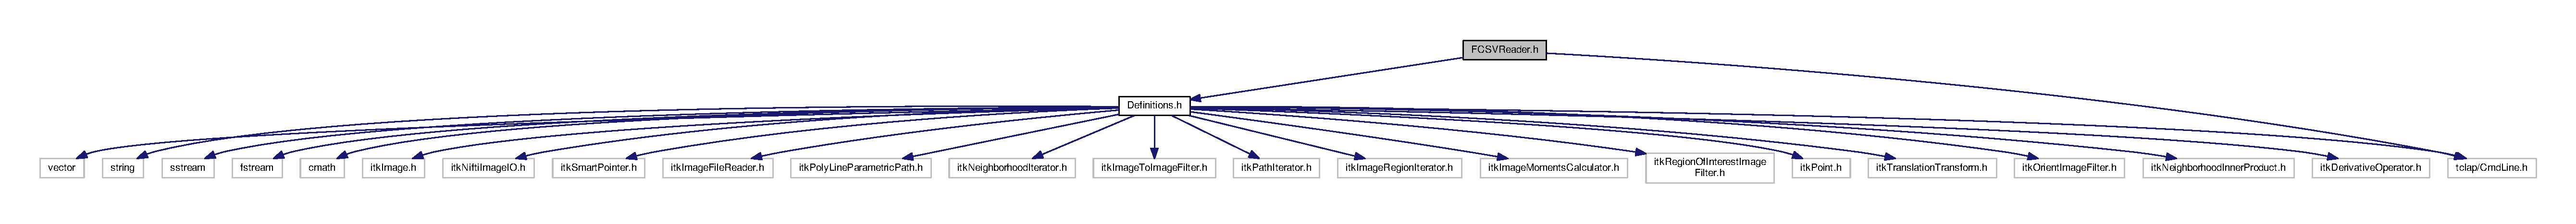
\includegraphics[width=350pt]{FCSVReader_8h__incl}
\end{center}
\end{figure}
\subsection*{Classes}
\begin{DoxyCompactItemize}
\item 
class \hyperlink{classFCSVReader}{F\-C\-S\-V\-Reader}
\end{DoxyCompactItemize}

\hypertarget{FCSVWriter_8h}{\section{F\-C\-S\-V\-Writer.\-h File Reference}
\label{FCSVWriter_8h}\index{F\-C\-S\-V\-Writer.\-h@{F\-C\-S\-V\-Writer.\-h}}
}
{\ttfamily \#include \char`\"{}Definitions.\-h\char`\"{}}\\*
{\ttfamily \#include \char`\"{}Abstract\-Writer.\-h\char`\"{}}\\*
{\ttfamily \#include $<$ostream$>$}\\*
{\ttfamily \#include $<$sstream$>$}\\*
Include dependency graph for F\-C\-S\-V\-Writer.\-h\-:
\nopagebreak
\begin{figure}[H]
\begin{center}
\leavevmode
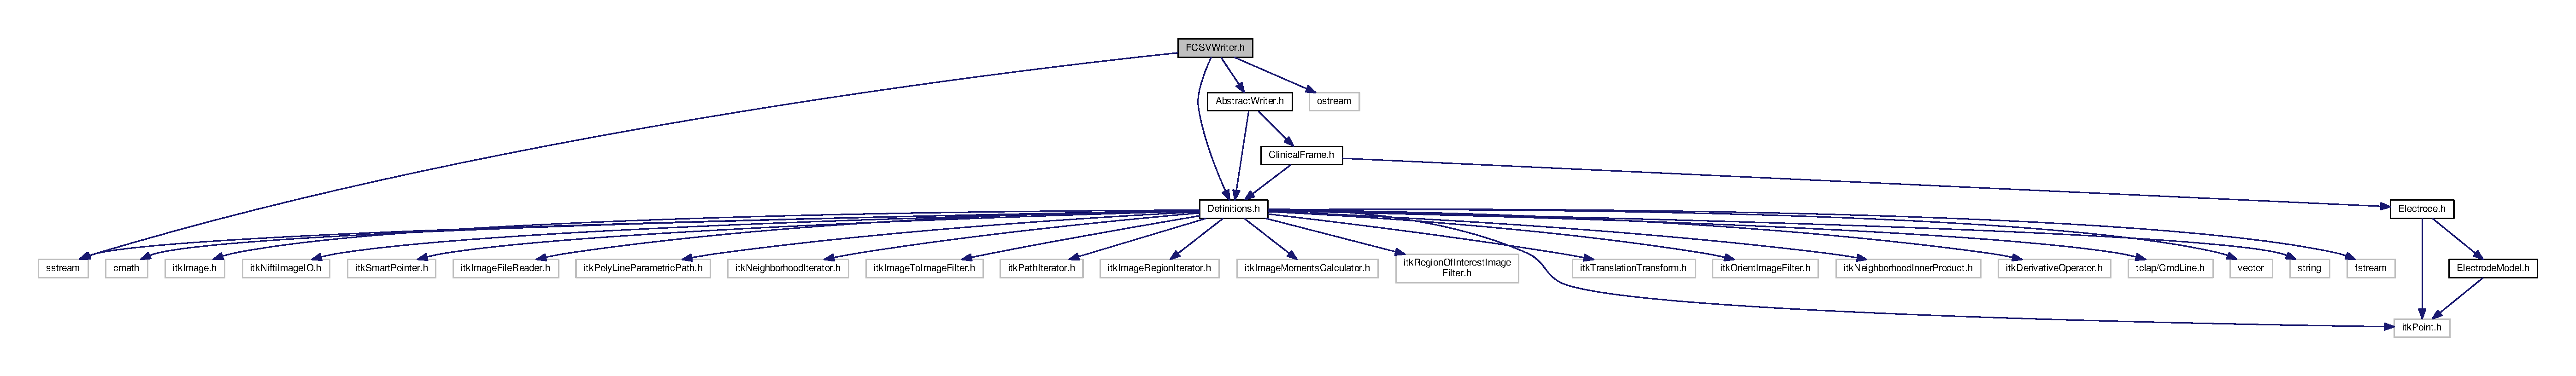
\includegraphics[width=350pt]{FCSVWriter_8h__incl}
\end{center}
\end{figure}
\subsection*{Classes}
\begin{DoxyCompactItemize}
\item 
class \hyperlink{classFCSVWriter}{F\-C\-S\-V\-Writer}
\end{DoxyCompactItemize}

\hypertarget{GMPIEstimator_8h}{\section{G\-M\-P\-I\-Estimator.\-h File Reference}
\label{GMPIEstimator_8h}\index{G\-M\-P\-I\-Estimator.\-h@{G\-M\-P\-I\-Estimator.\-h}}
}
\subsection*{Classes}
\begin{DoxyCompactItemize}
\item 
class \hyperlink{classGMPIEstimator}{G\-M\-P\-I\-Estimator}
\end{DoxyCompactItemize}

\hypertarget{VTKModelConstructor_8h}{\section{V\-T\-K\-Model\-Constructor.\-h File Reference}
\label{VTKModelConstructor_8h}\index{V\-T\-K\-Model\-Constructor.\-h@{V\-T\-K\-Model\-Constructor.\-h}}
}
{\ttfamily \#include \char`\"{}Definitions.\-h\char`\"{}}\\*
{\ttfamily \#include $<$vtk\-Append\-Poly\-Data.\-h$>$}\\*
{\ttfamily \#include $<$vtk\-Tube\-Filter.\-h$>$}\\*
{\ttfamily \#include $<$vtk\-Line\-Source.\-h$>$}\\*
{\ttfamily \#include $<$vtk\-Poly\-Data.\-h$>$}\\*
{\ttfamily \#include $<$vtk\-Parametric\-Spline.\-h$>$}\\*
{\ttfamily \#include $<$vtk\-Parametric\-Function\-Source.\-h$>$}\\*
{\ttfamily \#include $<$vtk\-Smart\-Pointer.\-h$>$}\\*
{\ttfamily \#include $<$vtk\-Poly\-Data\-Writer.\-h$>$}\\*
Include dependency graph for V\-T\-K\-Model\-Constructor.\-h\-:
\nopagebreak
\begin{figure}[H]
\begin{center}
\leavevmode
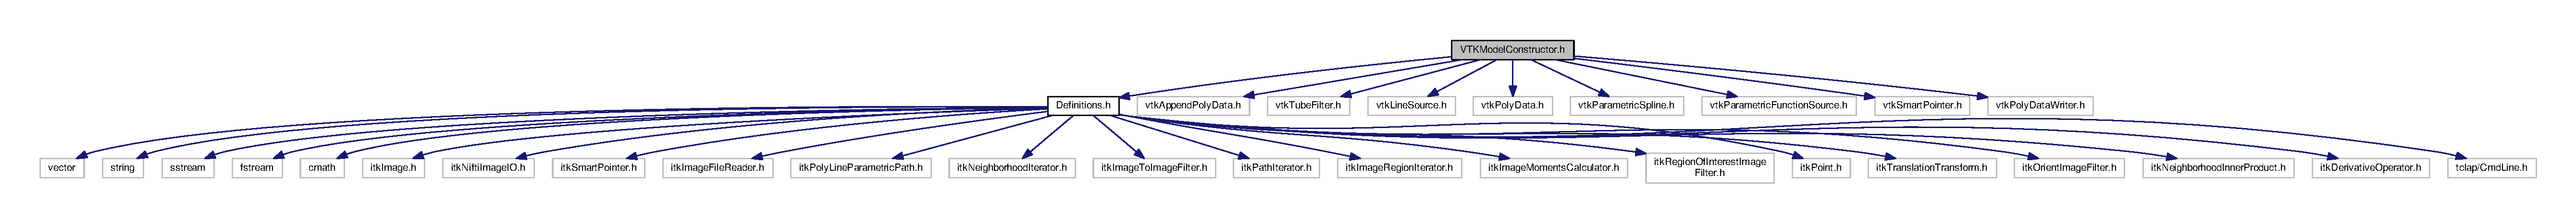
\includegraphics[width=350pt]{VTKModelConstructor_8h__incl}
\end{center}
\end{figure}
This graph shows which files directly or indirectly include this file\-:
\nopagebreak
\begin{figure}[H]
\begin{center}
\leavevmode
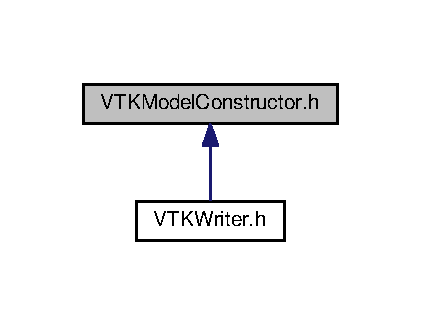
\includegraphics[width=202pt]{VTKModelConstructor_8h__dep__incl}
\end{center}
\end{figure}
\subsection*{Classes}
\begin{DoxyCompactItemize}
\item 
class \hyperlink{classVTKModelConstructor}{V\-T\-K\-Model\-Constructor}
\end{DoxyCompactItemize}

\hypertarget{VTKWriter_8h}{\section{V\-T\-K\-Writer.\-h File Reference}
\label{VTKWriter_8h}\index{V\-T\-K\-Writer.\-h@{V\-T\-K\-Writer.\-h}}
}
{\ttfamily \#include \char`\"{}Definitions.\-h\char`\"{}}\\*
{\ttfamily \#include \char`\"{}Abstract\-Writer.\-h\char`\"{}}\\*
{\ttfamily \#include \char`\"{}V\-T\-K\-Model\-Constructor.\-h\char`\"{}}\\*
{\ttfamily \#include $<$ostream$>$}\\*
{\ttfamily \#include $<$sstream$>$}\\*
Include dependency graph for V\-T\-K\-Writer.\-h\-:
\nopagebreak
\begin{figure}[H]
\begin{center}
\leavevmode
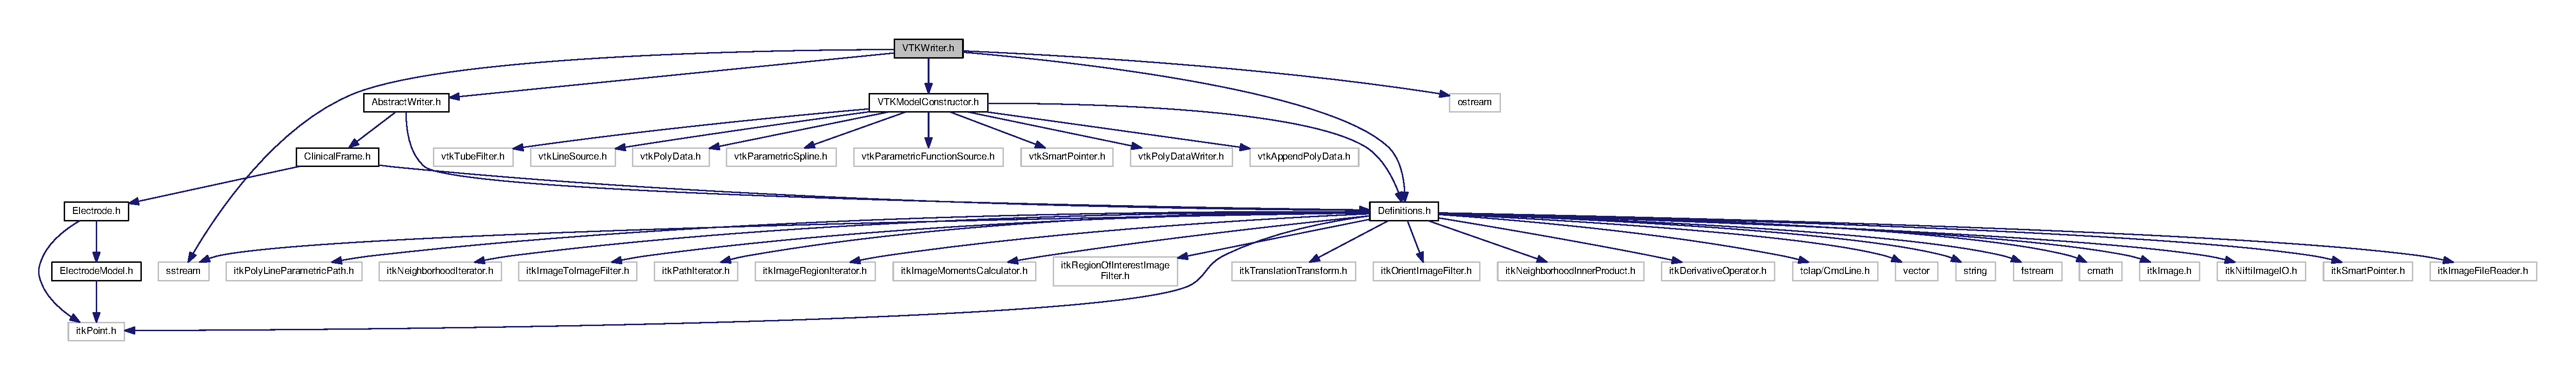
\includegraphics[width=350pt]{VTKWriter_8h__incl}
\end{center}
\end{figure}
\subsection*{Classes}
\begin{DoxyCompactItemize}
\item 
class \hyperlink{classVTKWriter}{V\-T\-K\-Writer}
\end{DoxyCompactItemize}

%--- End generated contents ---

% Index
\newpage
\phantomsection
\addcontentsline{toc}{chapter}{Index}
\printindex

\end{document}
